\documentclass[14pt]{article}
%Fonts and Math packages
\usepackage{amsmath,amssymb,amsfonts,amsthm,bm,bbm,cancel,wasysym}
%Graphics packages
\usepackage{epsfig,graphics,graphicx,epstopdf}
%Tabular packages
\usepackage{array,booktabs,colortbl,colordvi,multirow}
% Colors
\usepackage{colordvi,color,xcolor}
% Links
\usepackage{hyperref}
% Others
\usepackage{rotating}
\usepackage{authblk}

%This is the next version file

%------------------------------ TOM'S preamble --------------------
\usepackage{verbatim}
\usepackage{cite}
\usepackage{subfig}
\usepackage{setspace}
\usepackage{url}
\usepackage[percent]{overpic}
\usepackage{slashed}
\usepackage{authblk}
\usepackage{xspace}
\usepackage{fullpage}
\usepackage{hyperref}

% Commonly used things
\newcommand{\Fermi}[0]{\textit{Fermi}\xspace}
\newcommand{\gtlike}[0]{\lstinline!gtlike!\xspace}
\newcommand{\sigmav}[0]{\ensuremath{\langle \sigma v \rangle}\xspace}
\newcommand{\bbbar}[0]{\ensuremath{b \bar b}\xspace}

\newcommand{\sigv}[0]{\ensuremath{\langle\sigma v\rangle}\xspace}
\newcommand{\sigvm}[0]{\ensuremath{\langle\sigma v\rangle_{\rm{UL}}}\xspace}
\newcommand{\tsigv}[0]{\ensuremath{\langle\sigma v\rangle R^{2}}\xspace}

% Units
\newcommand{\unit}[1]{\ensuremath{\mathrm{\,#1}}\xspace}
\newcommand{\TeV}{\unit{TeV}}
\newcommand{\GeV}{\unit{GeV}}
\newcommand{\MeV}{\unit{MeV}}
\newcommand{\degree}{\unit{^{\circ}}}
\newcommand{\cm}{\unit{cm}}
\newcommand{\kpc}{\unit{kpc}}
\newcommand{\second}{\unit{s}}
\newcommand{\photons}{\unit{photons}}
\renewcommand{\photon}{\unit{photons}}
\newcommand{\ph}{\unit{photons}}
\newcommand*{\pt}{\ensuremath{p_{\text{T}}}}

% Reference
\newcommand{\Figref}[1]{Figure \ref{figs:#1}}
\newcommand{\Secref}[1]{Section \ref{sec:#1}}
\newcommand{\Subsecref}[1]{Section \ref{subsec:#1}}
\newcommand{\Eqnref}[1]{Eq.~(\ref{eqn:#1})}

\newcommand{\figref}[1]{figure \ref{figs:#1}}
\newcommand{\secref}[1]{section \ref{sec:#1}}
\newcommand{\subsecref}[1]{section \ref{subsec:#1}}
\newcommand{\eqnref}[1]{eq.~(\ref{eqn:#1})}

\def\tev{\,{\rm TeV}}
\def\gev{\,{\rm GeV}}
\def\ie{{\it i.e.}}
\def\eg{{\it e.g.}}
\def\etc{{\it etc}}
\def\etal{{\it et al.}}
\def\ibid{{\it ibid}.}

\def\to{\rightarrow}
\def\Fermi{\,{\it Fermi}}

\newskip\zatskip \zatskip=0pt plus0pt minus0pt
\def\matth{\mathsurround=0pt}
\def\lsim{\mathrel{\mathpalette\atversim<}}
\def\gsim{\mathrel{\mathpalette\atversim>}}
\def\atversim#1#2{\lower0.7ex\vbox{\baselineskip\zatskip\lineskip\zatskip
  \lineskiplimit 0pt\ialign{$\matth#1\hfil##\hfil$\crcr#2\crcr\sim\crcr}}}


%------------------------------Comments --------------------

\newcommand{\JH}[1]{{\color{green} \bf JLH~\![#1]}} % J. Hewett comments

\newcommand{\TR}[1]{{\color{red} \bf TR~\![#1]}} % T. Rizzo comments


%--------------------------- TEXT DIMENSIONS AND MARGINS ------------------------------%

\renewcommand{\topfraction}{1}
\renewcommand{\bottomfraction}{1}
\renewcommand{\textfraction}{0}
\renewcommand{\baselinestretch}{1.0}
\parskip=1.0ex
\setcounter{topnumber}{10}
\setcounter{bottomnumber}{10}
\setcounter{totalnumber}{10}

\textwidth=16cm
\textheight=23cm
\oddsidemargin=0.2cm
\evensidemargin=0.2cm

\author[1]{Clement Helsens}
\author[2]{David Jamin}
\author[3]{Michelangelo L. Mangano}
\author[4]{Thomas G. Rizzo}
\author[1]{Michele Selvaggi}

\affil[1]{CERN EP-Departement, CH-1211 Geneva 23, Switzerland}
\affil[2]{Academia Sinica, Institute of  Physics, Taipei, Taiwan}
\affil[3]{CERN TH-Departement, CH-1211 Geneva 23, Switzerland}
\affil[4]{SLAC National Accelerator Laboratory 2575 Sand Hill Rd., Menlo Park, CA, 94025 USA}

\title{$Z'$ identification at the HE-LHC} 

%------------------------------------- BEGIN DOCUMENT ------------------------------------------%

\begin{document}
\maketitle
\tableofcontents


%--------------------------------------------- ABSTRACT ---------------------------------------------%
\begin{abstract}
 
\noindent

The 14 TeV LHC with L=3 ab$^{-1}$ of integrated luminosity can search for new $Z'$ gauge bosons from the classic extended gauge theories up to masses 
of roughly $\simeq 6$ TeV.  Here we analyzed the capability of the 27 TeV HE-LHC with L=15 ab$^{-1}$ to distinguish among six $Z'$ models employing only 
the $e^+e^-$ and $\mu^+\mu^-$ channels assuming that $M_{Z'}=6$ TeV. Under the assumption that these $Z'$'s decay only to SM particles,  we show that 
there are sufficient observables to perform this model differentiation in most cases. 
\end{abstract}


%-------------------------------- DOCUMENT: INTRODUCTION ---------------------------------%

\section{Context of the study}
It is legitimate to assume that a heavy resonance could be seen at the end of High Luminosity LHC (HL-HLC). If that is the case a new collider with higher energy 
in the center of mass is needed to study its property as not enough events will be available at 14~TeV. In this document we present the discrimination potential of a High Energy LHC (HE-LHC)
with an assumed center of mass energy of 27~TeV.


\section{Bounds from HL-LHC}
As a starting point it is needed to understand what are, for $\sqrt s=14$ TeV, for the typical exclusion/discovery reaches for some standard reference $Z'$ models assuming L=3 ab$^{-1}$ 
employing only the $e^+e^-$ and $\mu^+\mu^-$ channels. To address this and the other questions below we will use the same set of $Z'$ models as employed 
in \cite{Rizzo:2014xma} and mostly in \cite{Han:2013mra}, both of which we will refer to frequently. We employ the MMHT2014 NNLO set \cite{Harland-Lang:2014zoa} 
throughout with an appropriate constant $K$-factor (=1.27) for numerics. 
The upper panel in Fig.~\ref{toy} shows the production cross section times leptonic BF for these models at 14 TeV in the NWA. It has 
been and will be assumed here that these $Z'$ states only decay to SM particles. 

Using the present ATLAS and CMS results at 13 TeV, \cite{Aaboud:2017buh} and \cite{Sirunyan:2018exx}, it is straightforward to estimate by extrapolation the eventual 14 TeV 
exclusion reach in the combined $e+\mu$ sample; this is given in the first column of Table~\ref{spec}. For discovery, only the $e$ channel is used due to poor $\mu$-pair mass 
resolution near $M_{Z'}=6$ TeV although the muons will add some additional support for any observed excess as large masses. Estimates of the $3\sigma$ evidence and $5\sigma$ 
discovery limits are also given in the Table. Based on these results, we will assume in our study below that we are dealing with a $Z'$ of mass 6 TeV; somewhat smaller mass 
choices will lead to very similar conclusions based on the ratio of predicted event rates shown in the lower panel of Fig.~\ref{toy}.  Fig.\ref{toy2} shows the NWA cross 
sections for the same set of models but now at 27 TeV; with L=15 ab$^{-1}$, we note that very large statistical samples will be available for the case of $M_{Z'}=6$ TeV 
for each dilepton channel. 


\begin{figure}[htbp]
  \centering
    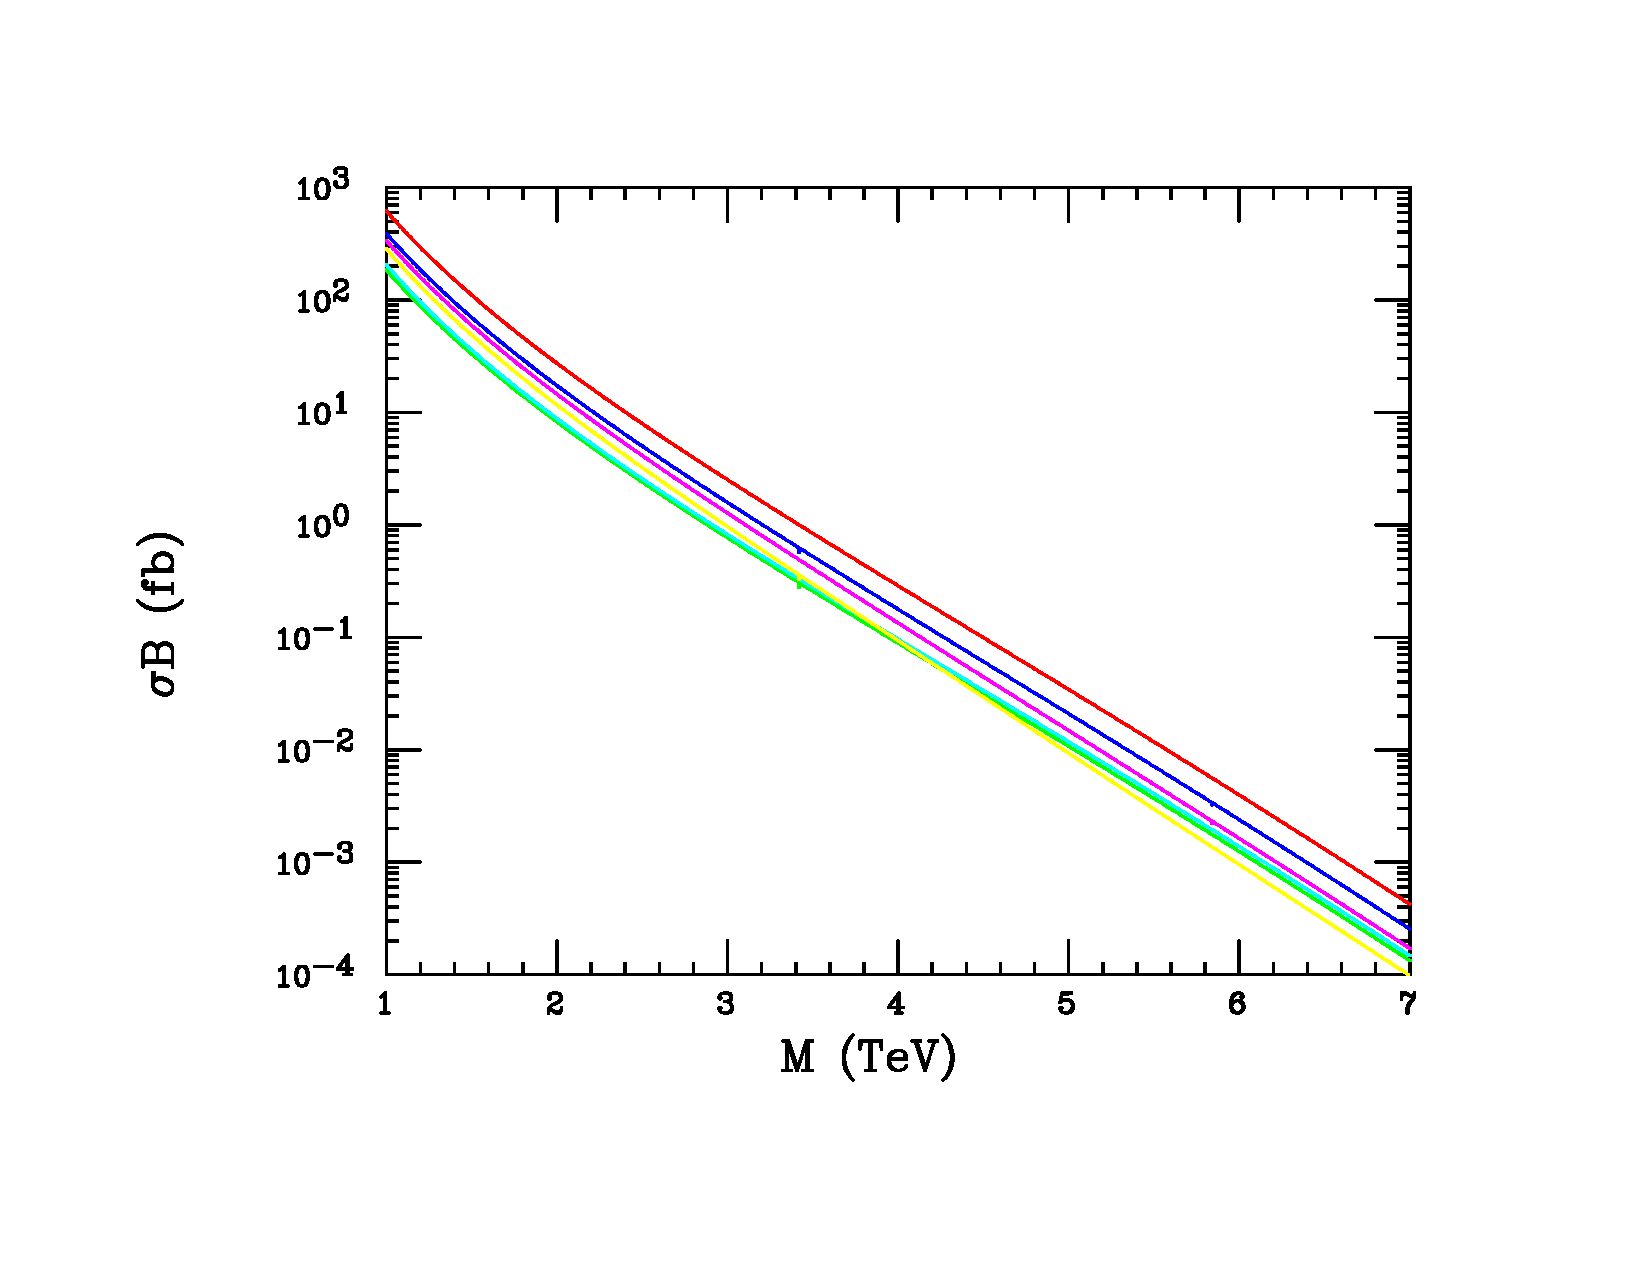
\includegraphics[trim={2cm 2cm 2cm 2cm},clip,width=0.49\columnwidth]{figures/zp14tev-ref.pdf}
    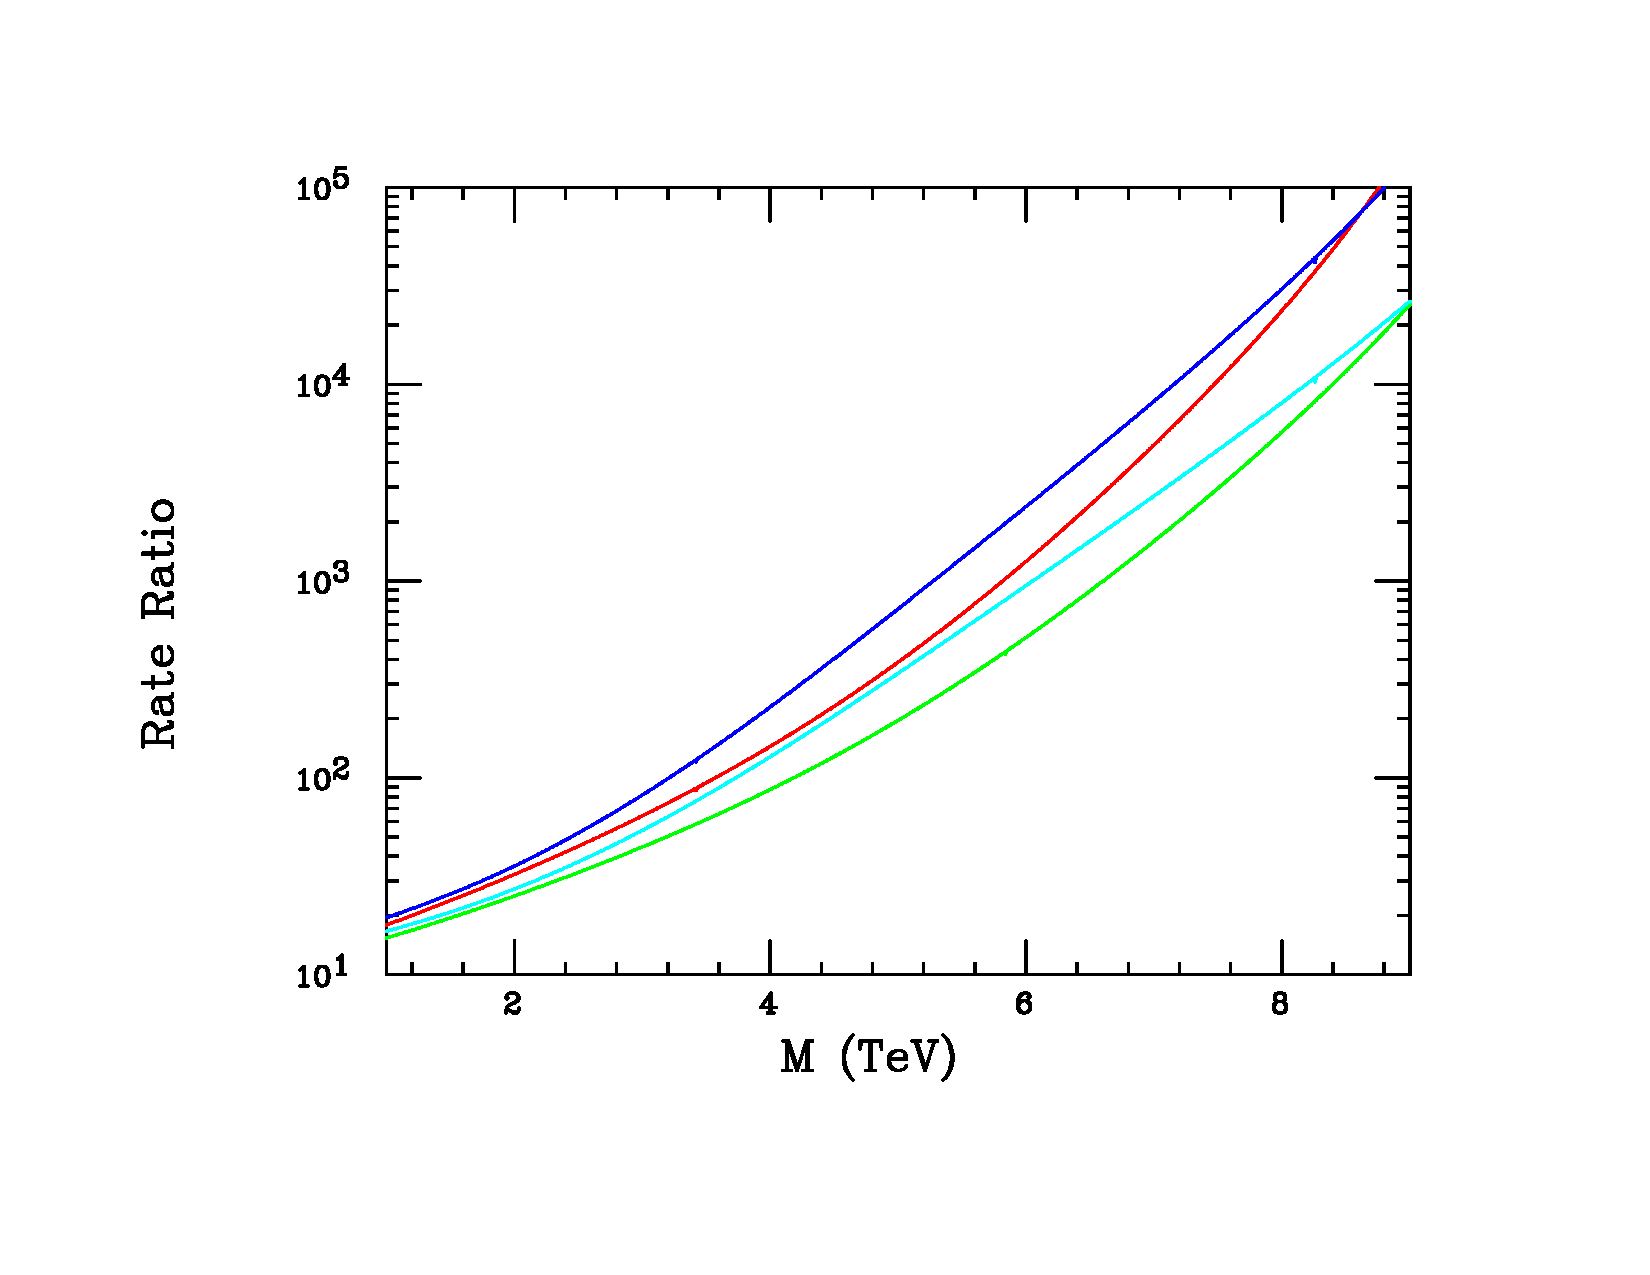
\includegraphics[trim={2cm 2cm 2cm 2cm},clip,width=0.49\columnwidth]{figures/scaled-ratio.pdf}
\caption{(Top) $\sigma B_l$ in the NWA for the $Z'$ production at the $\sqrt s=14$ TeV LHC as functions of the $Z'$ mass: SSM(red), LRM (blue), $\psi$(green), $\chi$(magenta), 
$\eta$(cyan), I(yellow).  (Bottom) Ratio of the number of events  for $\sqrt s=27$ TeV, L=15 ab$^{-1}$ to that at 13[14] TeV, L=3 ab$^{-1}$ for 
$\bar u u$ (red) and $\bar d d$ (blue)  [green, cyan] initial state partons with fixed invariant mass $M$.}
\label{toy}
\end{figure}



%
\begin{table}
\centering
\begin{tabular}{|l|c|c|c|} \hline\hline
  Model &   95$\%$ CL     &  $3\sigma$     &   $5\sigma$   \\
\hline
SSM    &     6.62     &  6.09        &  5.62     \\
LRM    &   6.39     & 5.85        & 5.39  \\
$\psi$    &  6.10   & 5.55   & 5.07  \\
$\chi$   &  6.22    & 5.68    & 5.26   \\
$\eta$   &  6.15     &  5.59  &  5.16   \\
~I        & 5.98   &  5.45   &  5.05  \\
\hline\hline
\end{tabular}
\caption{ $\sqrt s=14$ TeV results for $M_{Z'}$ in TeV as discussed in the text. }
\label{spec}
\end{table}
%


\section{Discrimination from direct calculations}
Question: Can we use just this dilepton channel to distinguish between these six $Z'$ models? 
\newline
\\
We make use of 3 observables, all in NWA: $\sigma B_l$, the forward-backward asymmetry, $A_{FB}$ and the rapidity ratio, $r_y$. These last two are defined 
and discussed at some extent in both \cite{Rizzo:2014xma} and \cite{Han:2013mra}.  Given the ATLAS and CMS analyses as presented in \cite{Han:2016qpd} 
and \cite{CMS:2017zzj} we employ the entire range of rapidity $|y|\leq 2.5$ in defining these quantities. Based on these same works and \cite{Han:2013mra}, 
In addition to usual statistical errors, we will assume a $2\%$ systematic error on the two ratios as most uncertainties (lumi and PDF) will cancel between numerators 
and denominators. For $\sigma B_l$, we assign a $5\%$ systematic error in addition to this $2\%$; all errors are then added in quadrature. I am aware that these may 
be aggressive numbers but the plots will tell all. 


\begin{figure}[htbp]
  \centering
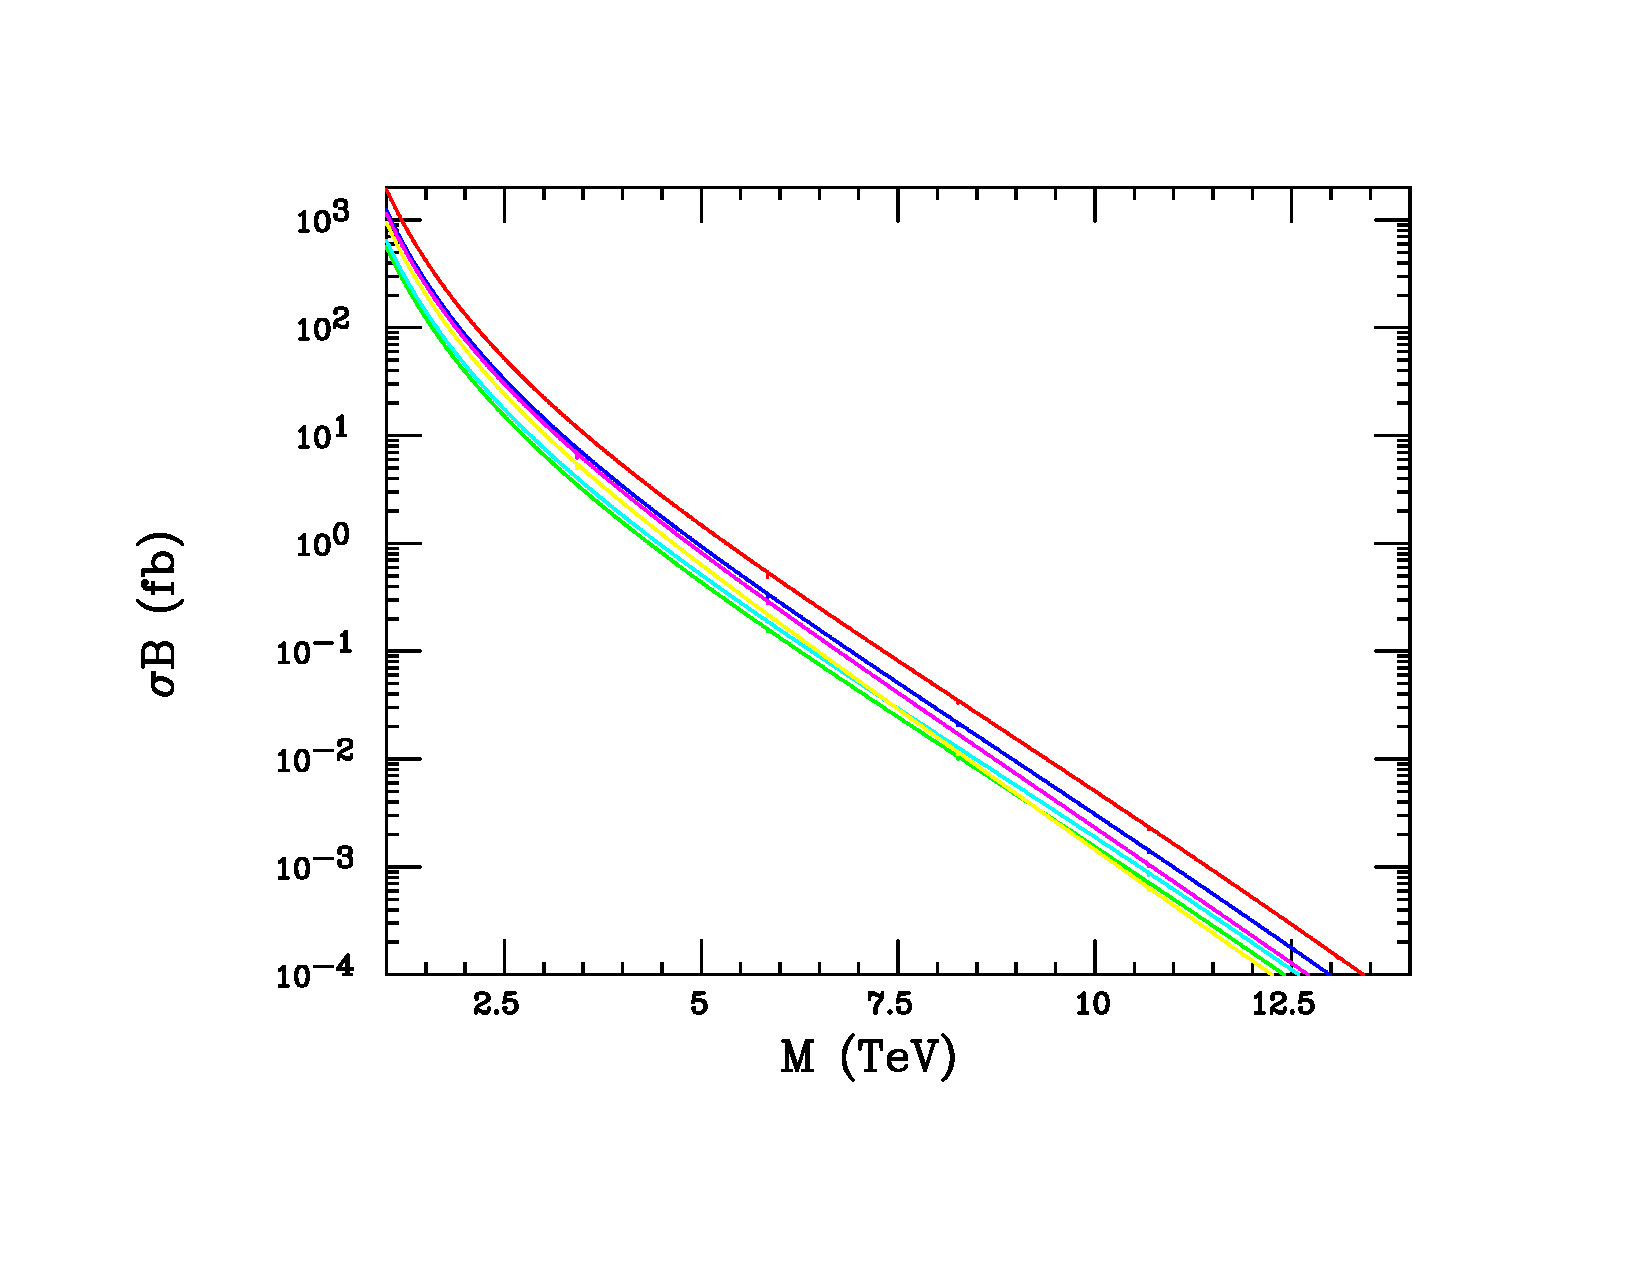
\includegraphics[trim={2cm 2cm 2cm 2cm},clip,width=0.49\columnwidth]{figures/zp27tev-ref.pdf}
\caption{ Same as the top panel in the previous Figure but now for the HE-LHC.}
\label{toy2}
\end{figure}



Fig.~\ref{toy3} shows the correlated predictions for these 3 observables for these six models given the above assumptions and employing {\it only} a single dilepton 
channel. Here we see that apart from a possible near degeneracy in models $\psi,\eta$, a reasonable $Z'$ model separation is indeed achieved. It is clear that this 
remains possible even with somewhat larger values for the systematic errors. I note again that the use of $\sigma B_l$ relies on the absence of new non-SM decay 
modes.



\begin{figure}[htbp]
  \centering
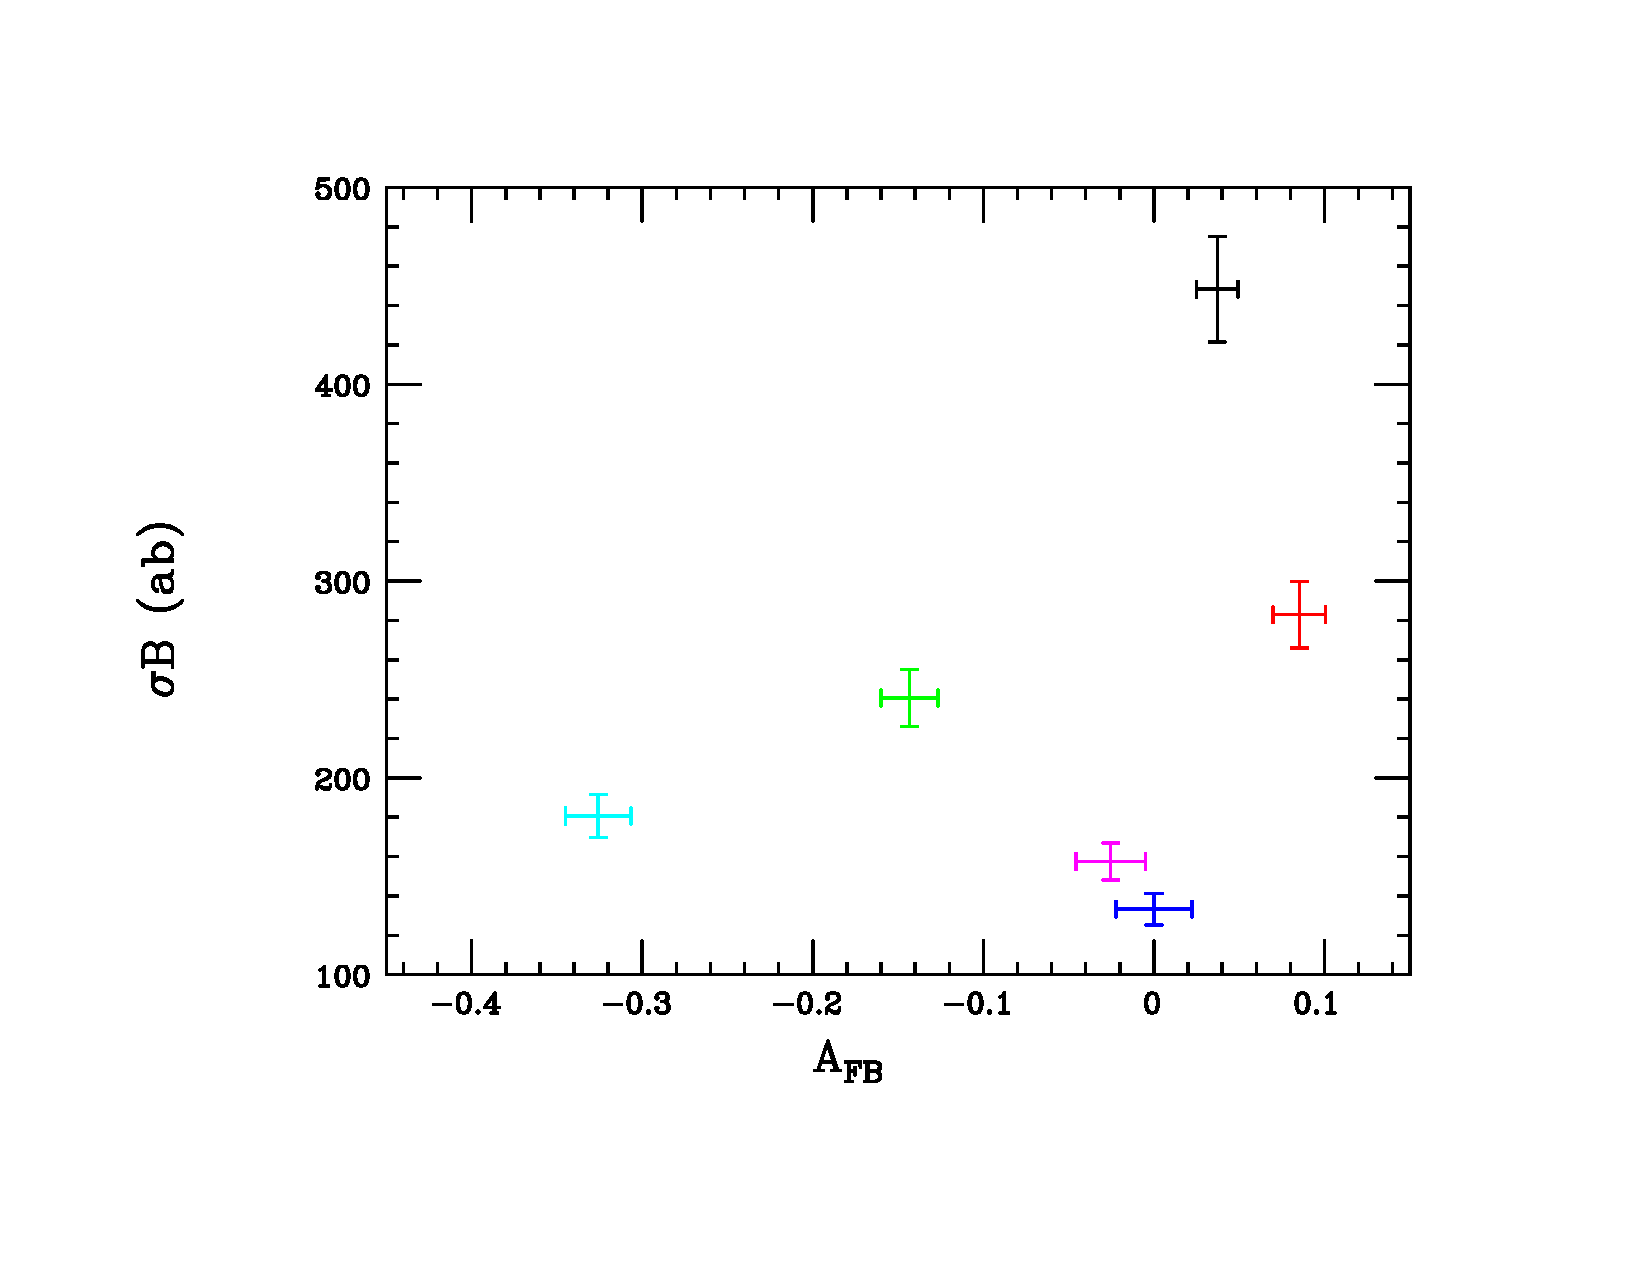
\includegraphics[trim={2cm 2cm 2cm 2cm},clip,width=0.49\columnwidth]{figures/compare2.pdf}
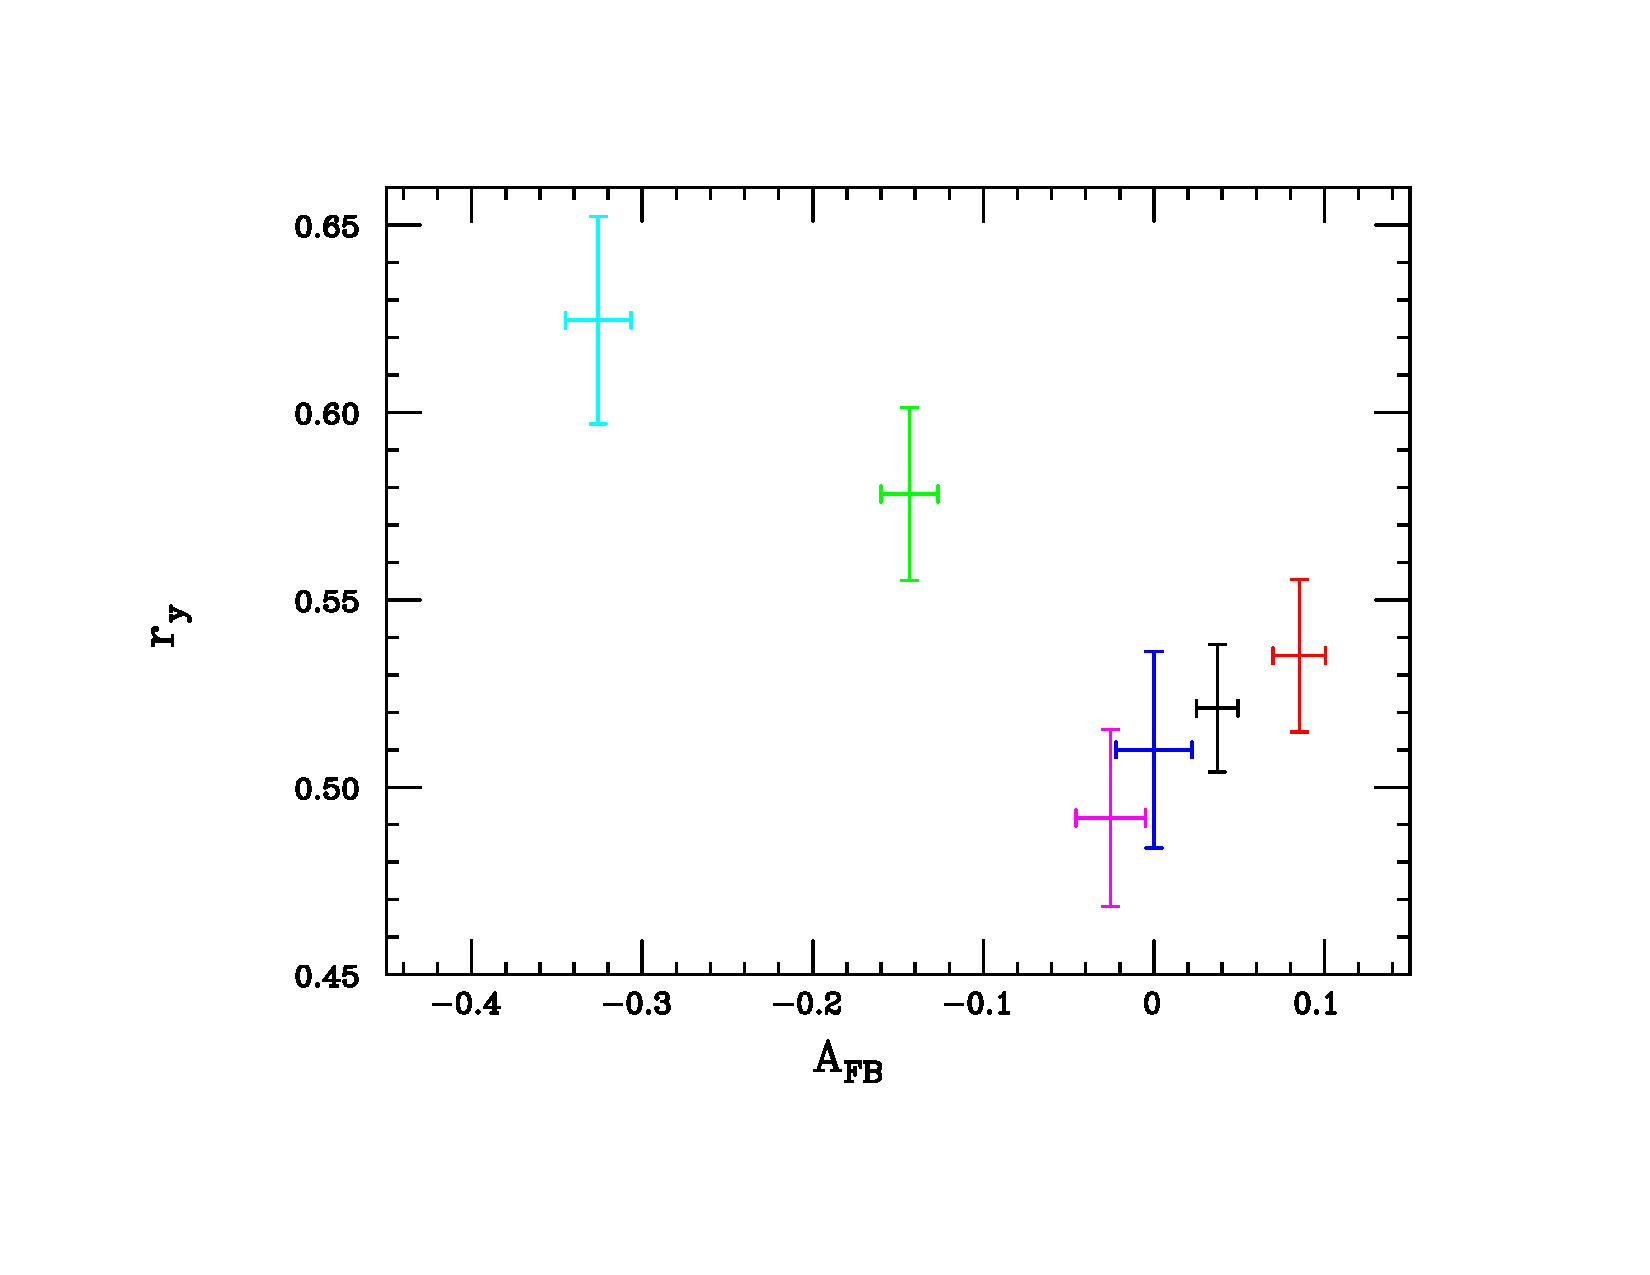
\includegraphics[trim={2cm 2cm 2cm 2cm},clip,width=0.49\columnwidth]{figures/compare3.pdf}
\caption{(Top) $\sigma B_l$ vs $A_{FB}$ and (Bottom) $r_y$ vs $A_{FB}$ at the HE-LHC assuming $M_Z'=6$ TeV as discussed in the text. 
SSM(black), LRM(red), $\psi$ (blue), $\chi$ (green), $\eta$ (magenta) and I (cyan). $1\sigma$ errors only are shown. }
\label{toy3}
\end{figure}




\section{Discrimination from detector level analysis}
The analyses presented in this section are all performed within the FCC software framework, FCCSW~\cite{fccsw}.
The detector parametrisation considered in this study is from HE-LHC official parametrisation for the yellow report~\cite{HELHCtwiki}.
The Monte Carlo are first presented in Section~\ref{subsection:MC} Leptonic decays are presented in~\ref{subsection:lepana}, and hadronic analyses in~\ref{subsection:hadana}.


\subsection{Monte Carlo Samples}
\label{subsection:MC}
Monte Carlo~(MC) simulated event samples were used to simulate the response of the FCC detector to signal and backgrounds. The muon momentum resolution 
is assumed to be $\sigma(p)/p \approx 20\%$ at $\pt= 20 $TeV. Signals are generated with {\scshape Pythia}~8.230~\cite{Sjostrand:2014zea} using the leading 
order cross-section from the generator. All lepton flavour decays of the $Z'$ are generated assuming universality of the couplings.
The Drell-Yan background has been generated using {\scshape MG5\_}a{\scshape MC@NLO}~2.5.2~\cite{Alwall:2014hca} at leading order only. 
A k-factor of 2 is applied to all the background processes.



\subsection{Leptonic analysis}
\label{subsection:lepana}
\subsubsection{Event selection and discovery potential}

Events are required to contain at least two same flavour leptons of opposite charge with $\pt > 500$~GeV, $|\eta|<$4.5. 
When mentioned a smaller acceptance of $|\eta|<$2.5 is considered to test the impact on the reduction of the statistics. 
An additional cut on the di-lepton invariant mass $m_{ll}>1$~TeV is applied to remove the low mass Drell-Yan. 
Figure~\ref{figure:lepana:mass} shows the invariant mass for a 6~TeV signal for the $ee$ (left) and $\mu\mu$ channels (right). 
The mass resolution is better for the ee channel, as expected from the higher performance of the electro-magnetic calorimeter at high energy.

\label{sec:lepana}
\begin{figure}[h]
  \centering
    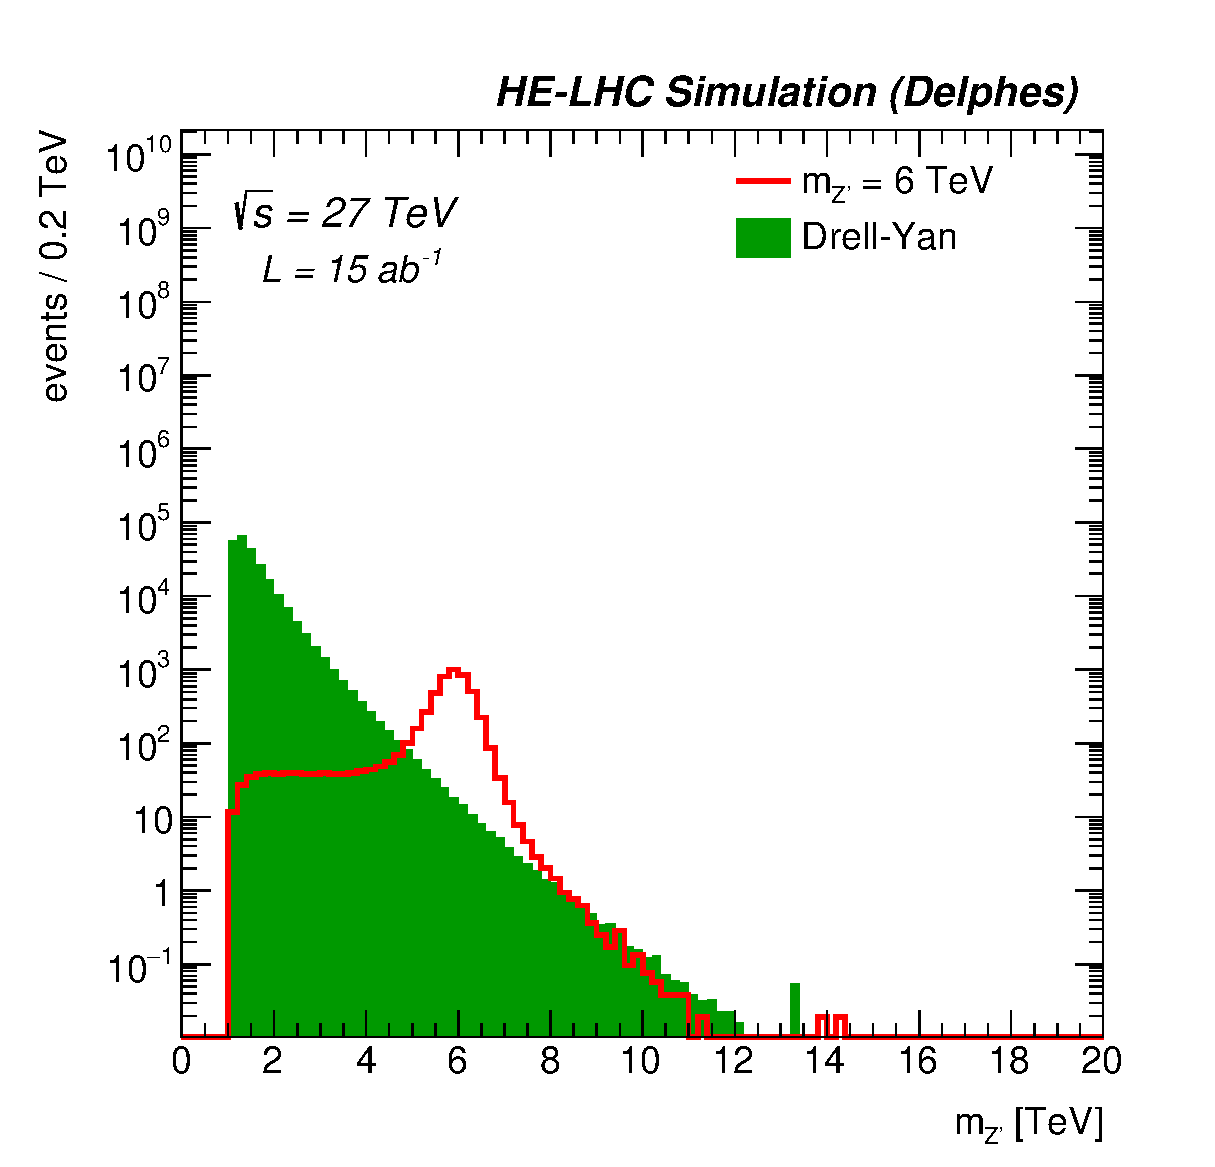
\includegraphics[width=0.45\columnwidth]{figures/Zpmumu_mzp_sel0_nostack_log.eps}
    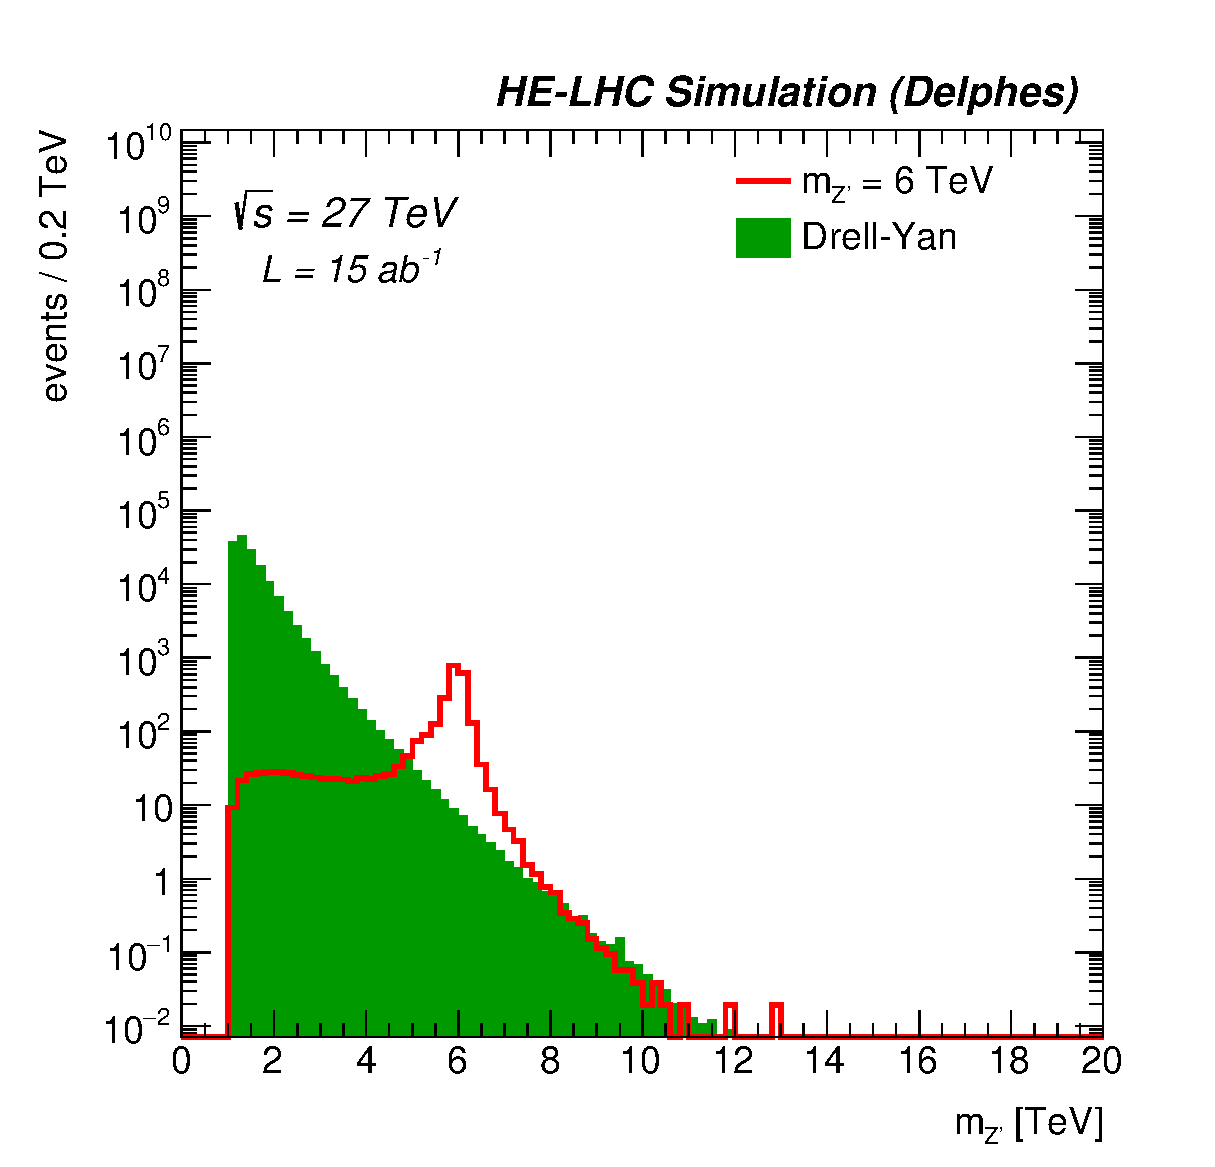
\includegraphics[width=0.45\columnwidth]{figures/Zpee_mzp_sel0_nostack_log.eps}
   \caption{Invariant mass for a 6~TeV signal after full event selection for ee channel (left) and $\mu\mu$ channel (right).}
  \label{figure:lepana:mass}
\end{figure}

Limits and discovery potential for di-lepton resonances are shown in Figure~\ref{figure:lepana:limdisc}. With the full 15~ab$^{-1}$ 
integrated luminosity, it is expected to exclude heavy $Z'$ resonances from 10 to 12.5~TeV depending on the model and discover 
a $Z'_{SSM}$ up to 12~TeV.

\begin{figure}[!htb]
  \centering
  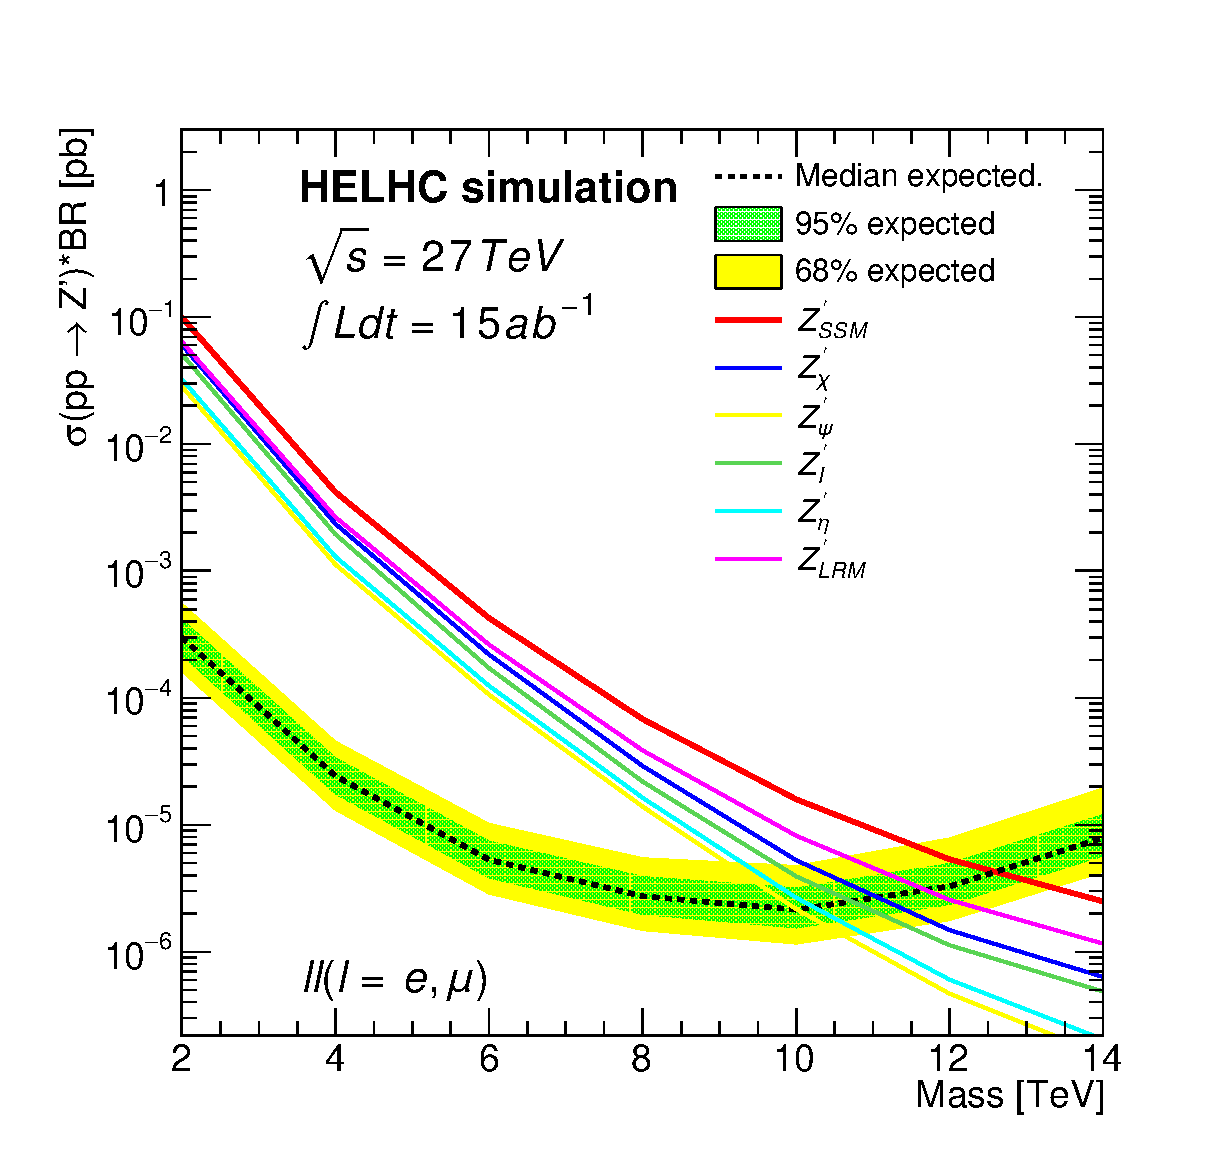
\includegraphics[width=0.45\columnwidth]{figures/lim_Zprime_ll_helhc_v01_allxs.eps}
  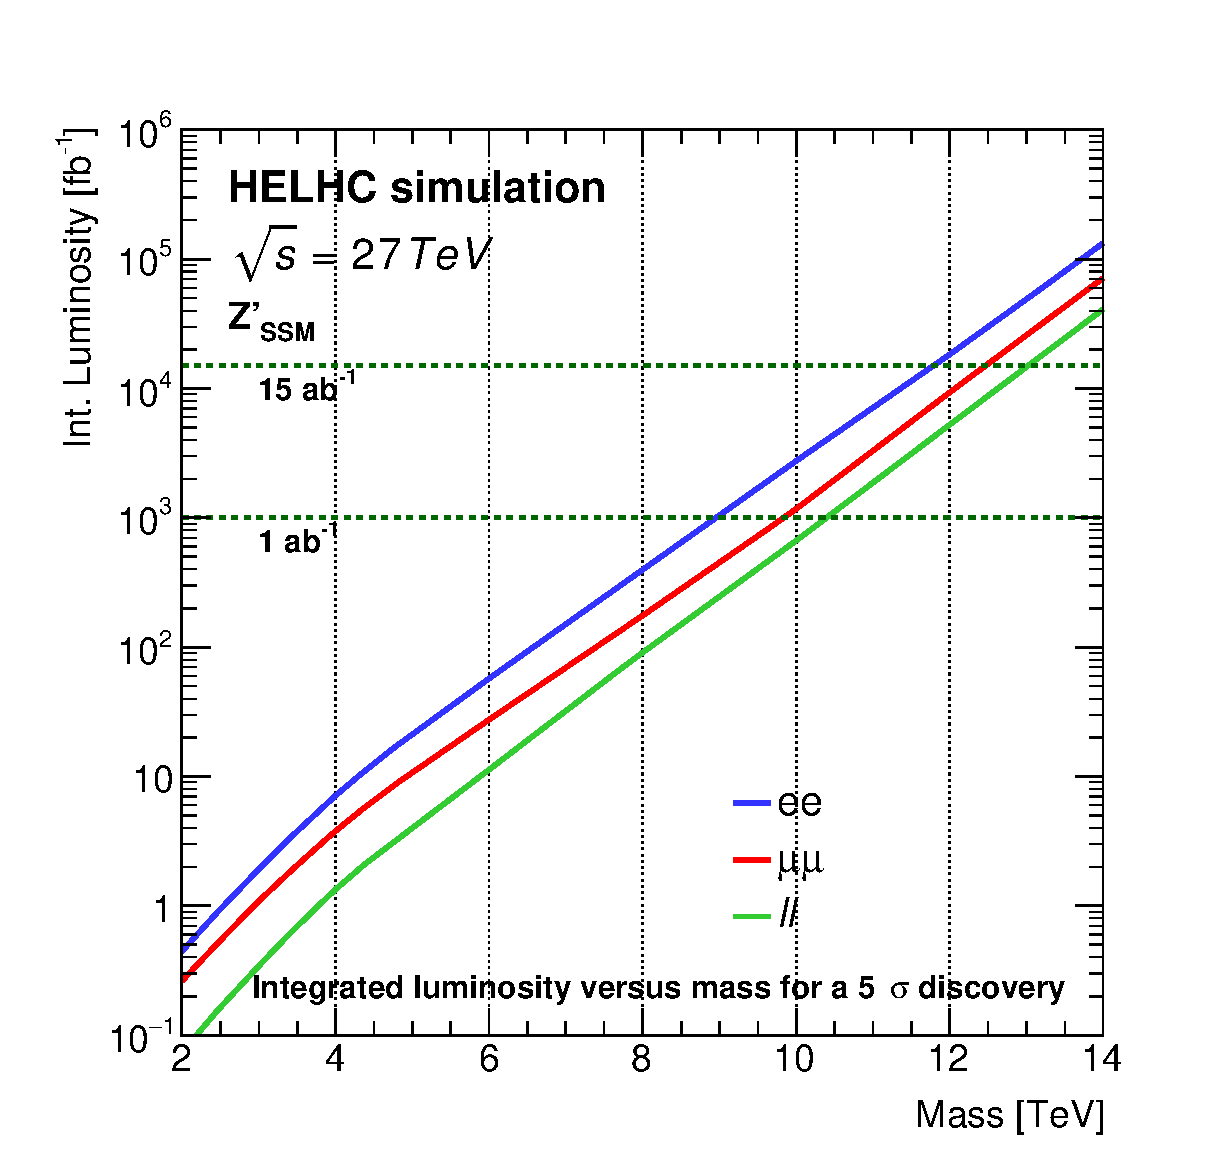
\includegraphics[width=0.45\columnwidth]{figures/DiscoveryPotential_ll_comb_rootStyle.eps}
  \caption{Limit versus mass for the di-lepton channel (left) and luminosity for a $5\sigma$ discovery (right) for the ee and $\mu\mu$ combined channels. }
  \label{figure:lepana:limdisc}
\end{figure}


\subsubsection{Variables definition}
\label{subsubsection:vardef}

As for the analysis from direct calculation, the observables are defined at the detector level. On Figure~\ref{figure:lepana:yzp} the 
rapidity of the $Z'$ is displayed, and as expected it is much more central for the signal than for the Drell-Yan background.

\begin{figure}[!htb]
  \centering
  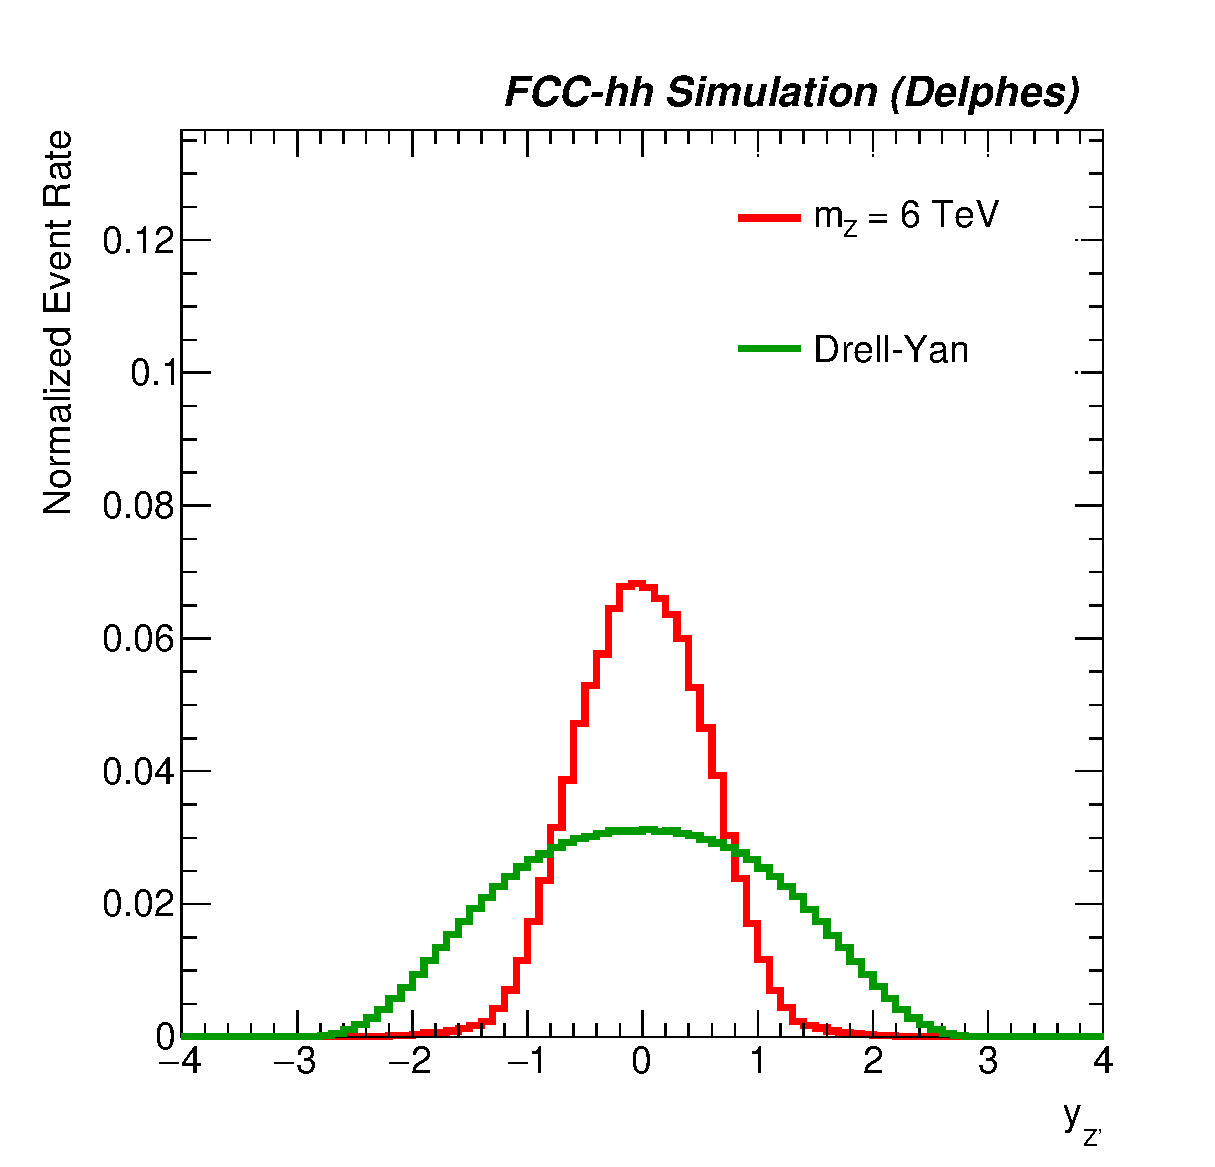
\includegraphics[width=0.45\columnwidth]{figures/yzp_sel0_lin_norm_ee.eps}
  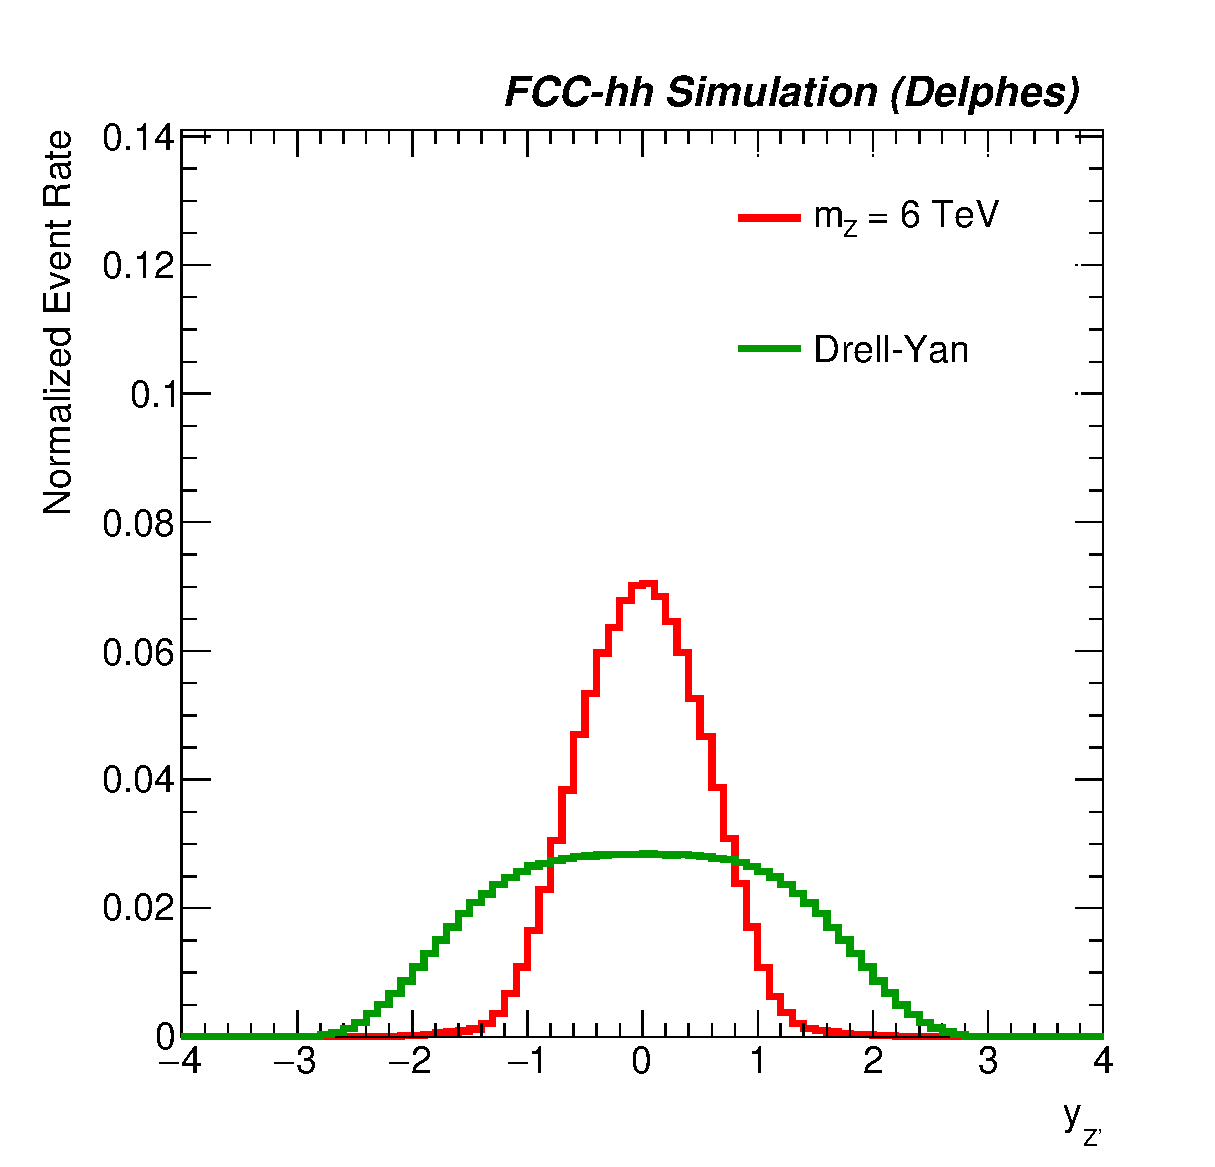
\includegraphics[width=0.45\columnwidth]{figures/yzp_sel0_lin_norm_mumu.eps}
  \caption{$Z'$ rapidity distribution comparing a 6~TeV signal and Drell-Yan background for ee (left) and $\mu\mu$ channels (right).}
  \label{figure:lepana:yzp}
\end{figure}

At detector level the variable $r_y$ is defined as the ratio of central over forward events:
\begin{equation}
r_y = \frac{\sigma(|y_{Z'}| < y_1)}{\sigma(y_1 < |y_{Z'}| <y_2)}
\end{equation}
with $y_1=0.5$ and $y_2=2.5$ for this study.

The variable $A_{FB}$ can be seen as a measure of the charge asymmetry
\begin{equation}
A_{FB} = A_C =  \frac{\sigma(\Delta|y| > 0) - \sigma(\Delta|y| < 0)}{\sigma(\Delta|y| > 0) + \sigma(\Delta|y| < 0)}
\end{equation}
where $\Delta|y| = |y_l| - |y_{\bar{l}}|$. It has been checked that this definition is equivalent to defining 
\begin{equation}
A_{FB} =   \frac{\sigma_F - \sigma_B}{\sigma_F + \sigma_B}
\end{equation}
with $\sigma_F = \sigma (cos\theta^{*}_{cs})>0$ and $\sigma_B = \sigma (cos\theta^{*}_{cs})<0$ and defining $\theta^*$ in the Collins-Soper 
frame as
\begin{equation}
cos\theta^{*}_{cs} =  \frac{Q_z}{|Q_z|} \frac{2(P_l^+P_{\bar{l}}^- - P_l^-P_{\bar{l}}^+)}{|Q| \sqrt{Q^2+Q^2_T}}
\end{equation}
where $Q$, $Q_T$ and $Q_z$ are the four-momentum, the transverse momentum, and the longitudinal
momentum of the di-lepton pair. $P_{l}(P_{\bar{l}})$ represents the four momenta of the lepton (anti-lepton),
and $P^\pm_l = (P^0_l \pm P^3_l)$.


\subsubsection{Optimisations}
\label{subsubsection:opti}
In Figure~\ref{figure:lepana:afb_dm} is represented $A_{FB}$ verus the acceptance window around a 6TeV signal. 
It is shown for signal only (top-left) and is flat as expected. Once background is introduced without uncertainties (top-right), and when the window 
becomes too large the asymmetry is diluted. When adding a 10\% uncertainty on the background (bottom-left) we observe as expected larger errors and quicker dilution.
The last plot (bottom-left) shows the same variable, but considering the full interference between the signal and the Drell-Yann. One can immediately 
note the fact that the dilution goes in opposite direction as when not considering the interference. 

\begin{figure}[!htb]
  \centering
   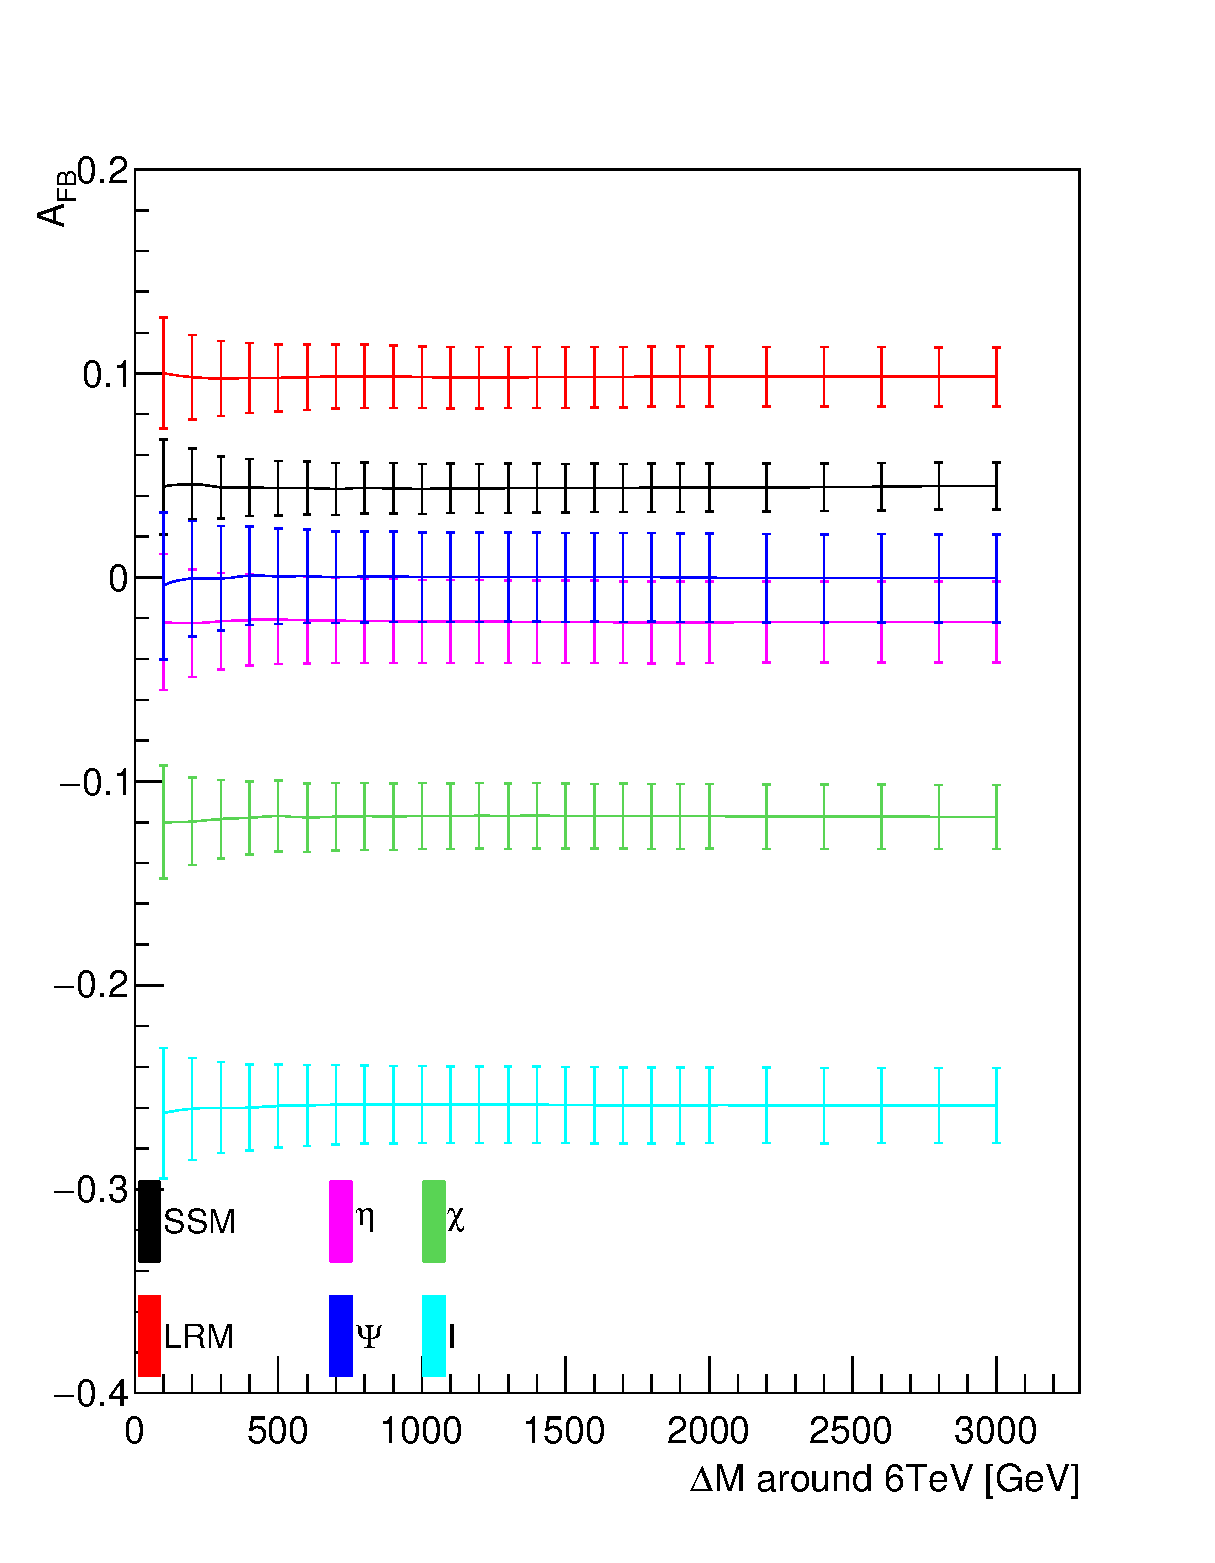
\includegraphics[width=0.45\columnwidth]{figures/afb_vs_dm_nobg.eps}
   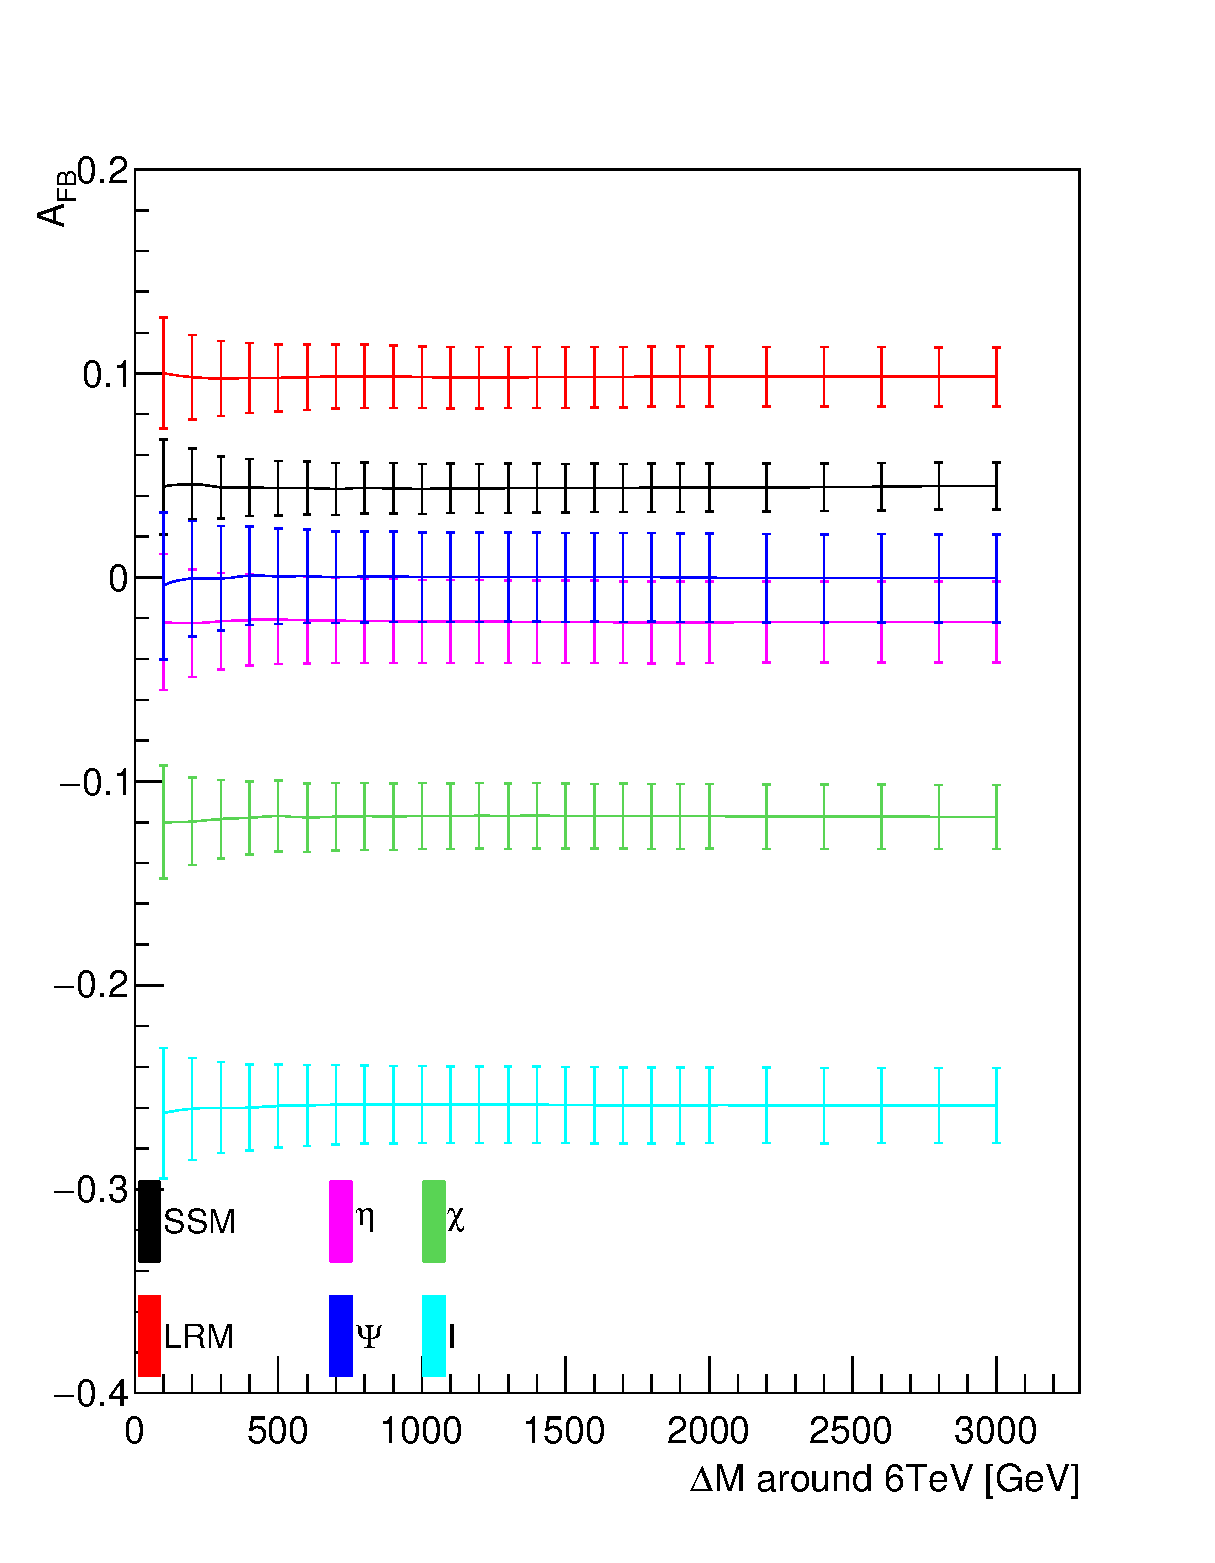
\includegraphics[width=0.45\columnwidth]{figures/afb_vs_dm_0p.eps}
   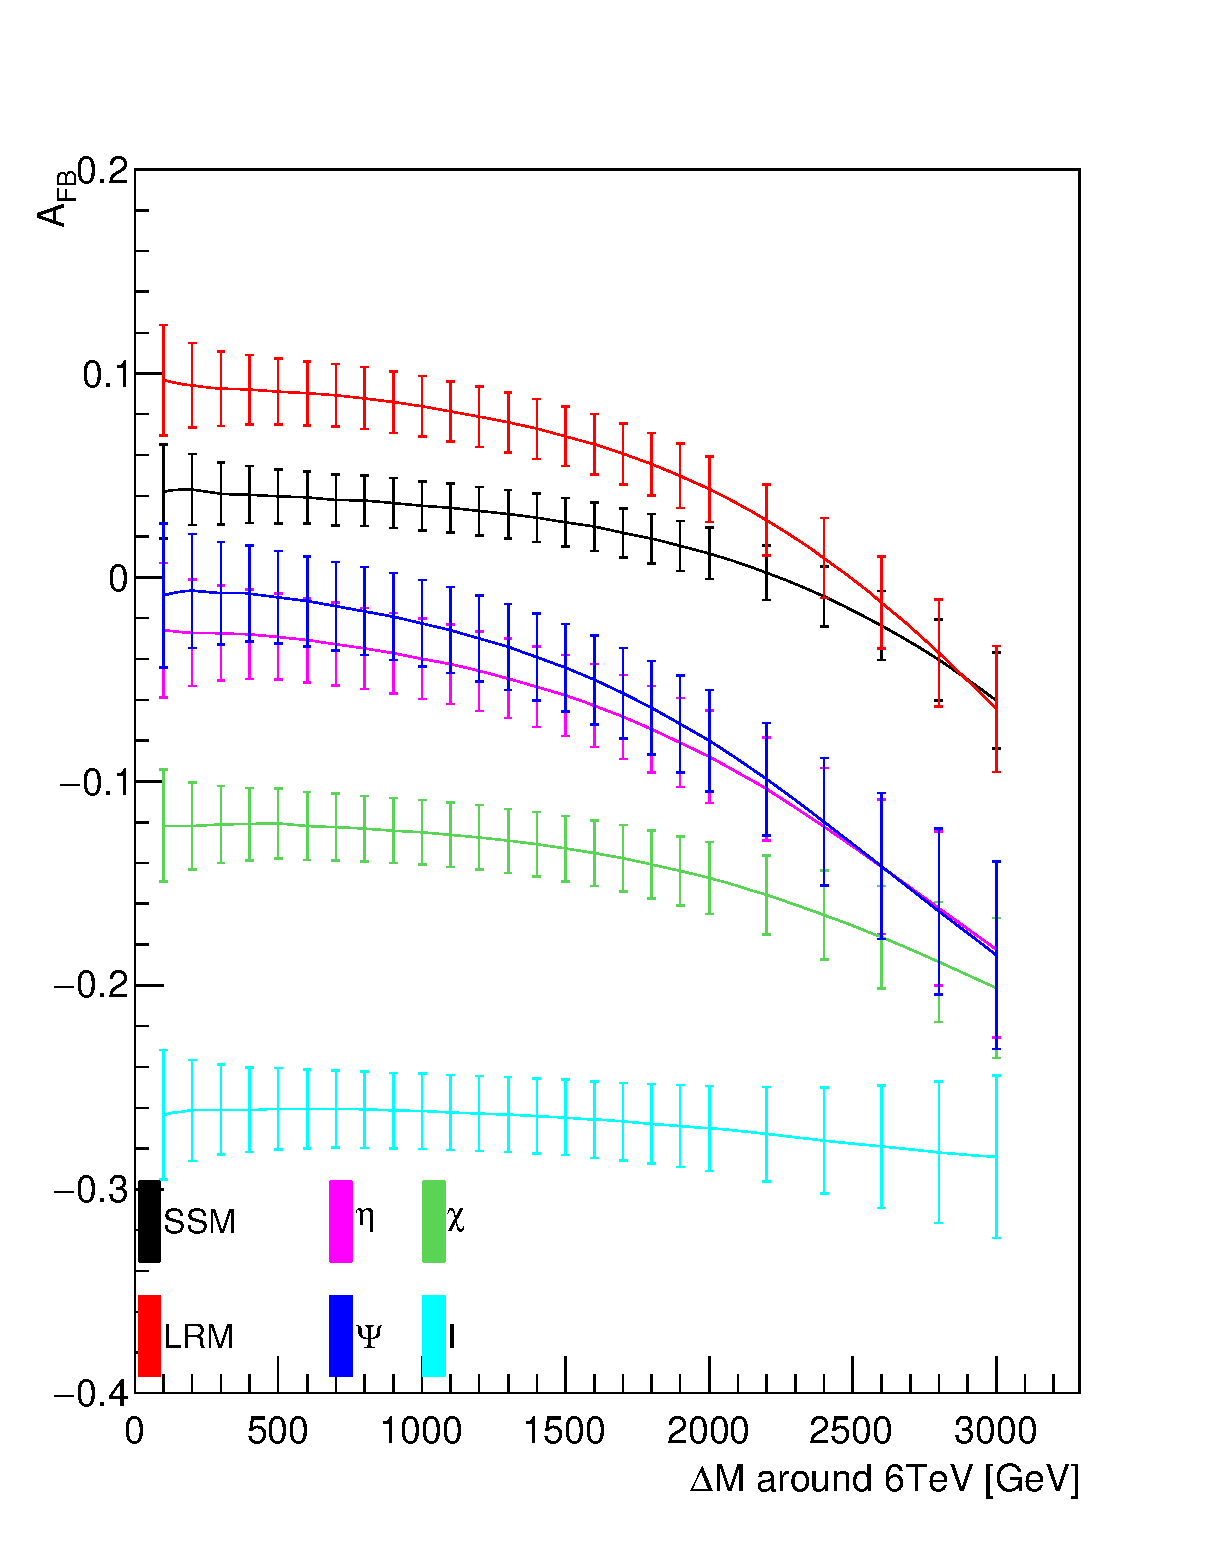
\includegraphics[width=0.45\columnwidth]{figures/afb_vs_dm_10p.eps}
   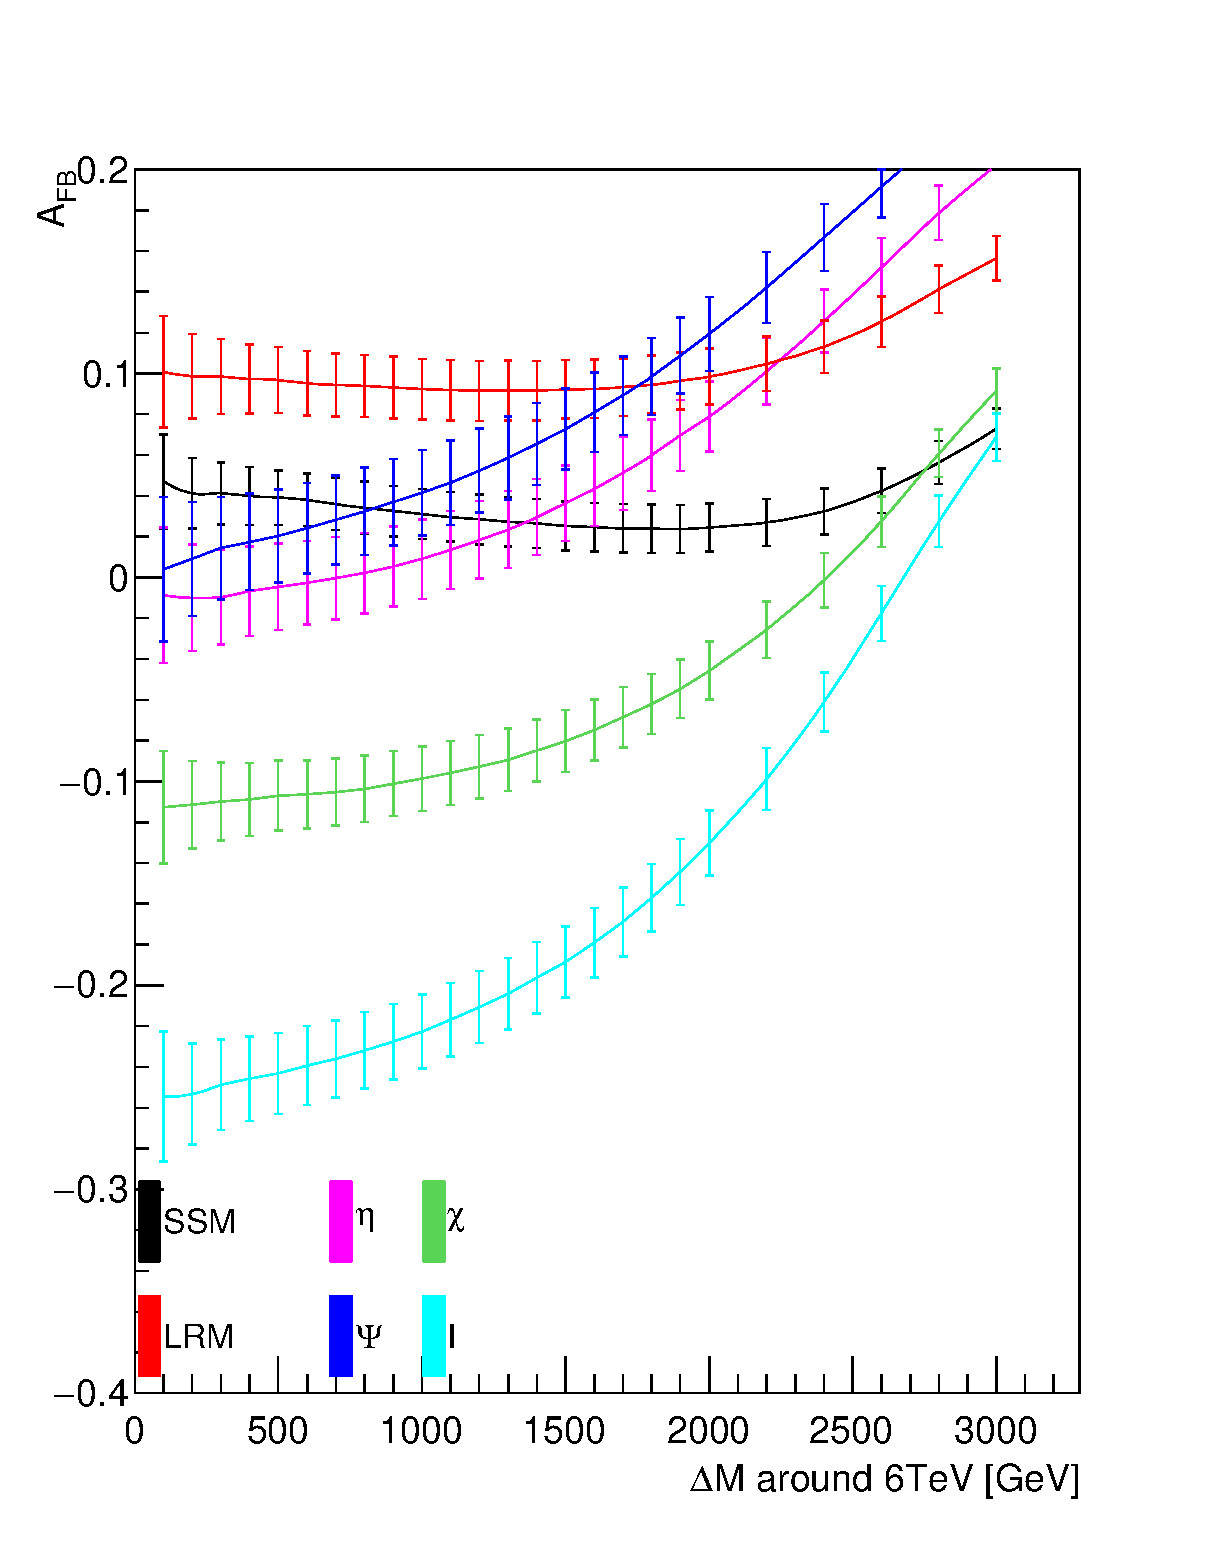
\includegraphics[width=0.45\columnwidth]{figures/afb_vs_dm_interf.eps}
  \caption{$A_{FB}$ versus invariant mass range around 6TeV considering no backgrounds (top left), backgrounds with no uncertainties (top right), backgrounds with 10\% uncertainties (bottom left) and full interference (bottom right).}
  \label{figure:lepana:afb_dm}
\end{figure}


\subsubsection{Results}
\label{subsubsection:results}
TODOBEGING\\
show cross section versus int luminosity, show error on AFB ry for models (2D), show scan lumi for hard to distinguish model, table that shows this impact of the eta, ISR, FSR, etc...
plot that shows how AFB and ry evolves with the deltaM cut
Show the effect of a cut a different cut on ry
TODOEND\\

\begin{table}
\centering
\begin{tabular}{| c | c | c | c | c | c | c | c | c | c | c | c |} \hline\hline
 & \multicolumn{2}{c|}{nominal}  & \multicolumn{2}{c|}{$|\eta|<4.5$} & \multicolumn{2}{c|}{no FSR} & \multicolumn{2}{c|}{no ISR} & \multicolumn{2}{c|}{Full interference}\\

\hline
  Model &  $A_{FB}$   &  $r_y$   &  $A_{FB}$   &  $r_y$&  $A_{FB}$   &  $r_y$&  $A_{FB}$   &  $r_y$&  $A_{FB}$   &  $r_y$ \\
\hline
SSM    &     6.62     &  6.09   &     6.62     &  6.09&     6.62     &  6.09&     6.62     &  6.09&     6.62     &  6.09      \\
LRM    &   6.39       &  6.09   &     6.62     &  6.09&     6.62     &  6.09&     6.62     &  6.09&     6.62     &  6.09 \\
$\psi$    &  6.10   &  6.09   &     6.62     &  6.09&     6.62     &  6.09&     6.62     &  6.09&     6.62     &  6.09   \\
$\chi$   &  6.22    &  6.09   &     6.62     &  6.09&     6.62     &  6.09&     6.62     &  6.09&     6.62     &  6.09    \\
$\eta$   &  6.15     &  6.09   &     6.62     &  6.09&     6.62     &  6.09&     6.62     &  6.09&     6.62     &  6.09    \\
~I        & 5.98   &  6.09   &     6.62     &  6.09&     6.62     &  6.09&     6.62     &  6.09&     6.62     &  6.09   \\
\hline\hline
\end{tabular}
\caption{$A_{FB}$ and $r_y$ values for different models and different assumptions.}
\label{tab:leptonicresonances:comp}
\end{table}

We have checked that increasing the acceptance of the leptons to 4.5 in pseudo-rapidity did not improved the discrimination further. 
Using a profile likelihood technique, the signal strength $\mu$ can be fitted together with its corresponding error. 


\subsection{Hadronic analysis}
\label{subsection:hadana}
In this section the hadronic decays of the $Z'$ will be tested in order to enhance the discrimination potential. 

\subsubsection{$Z' \rightarrow t\bar{t}$}
\subsubsection{$Z' \rightarrow b\bar{b}$}
\subsubsection{$Z' \rightarrow q\bar{q}$}

\begin{figure}[h]
  \centering
  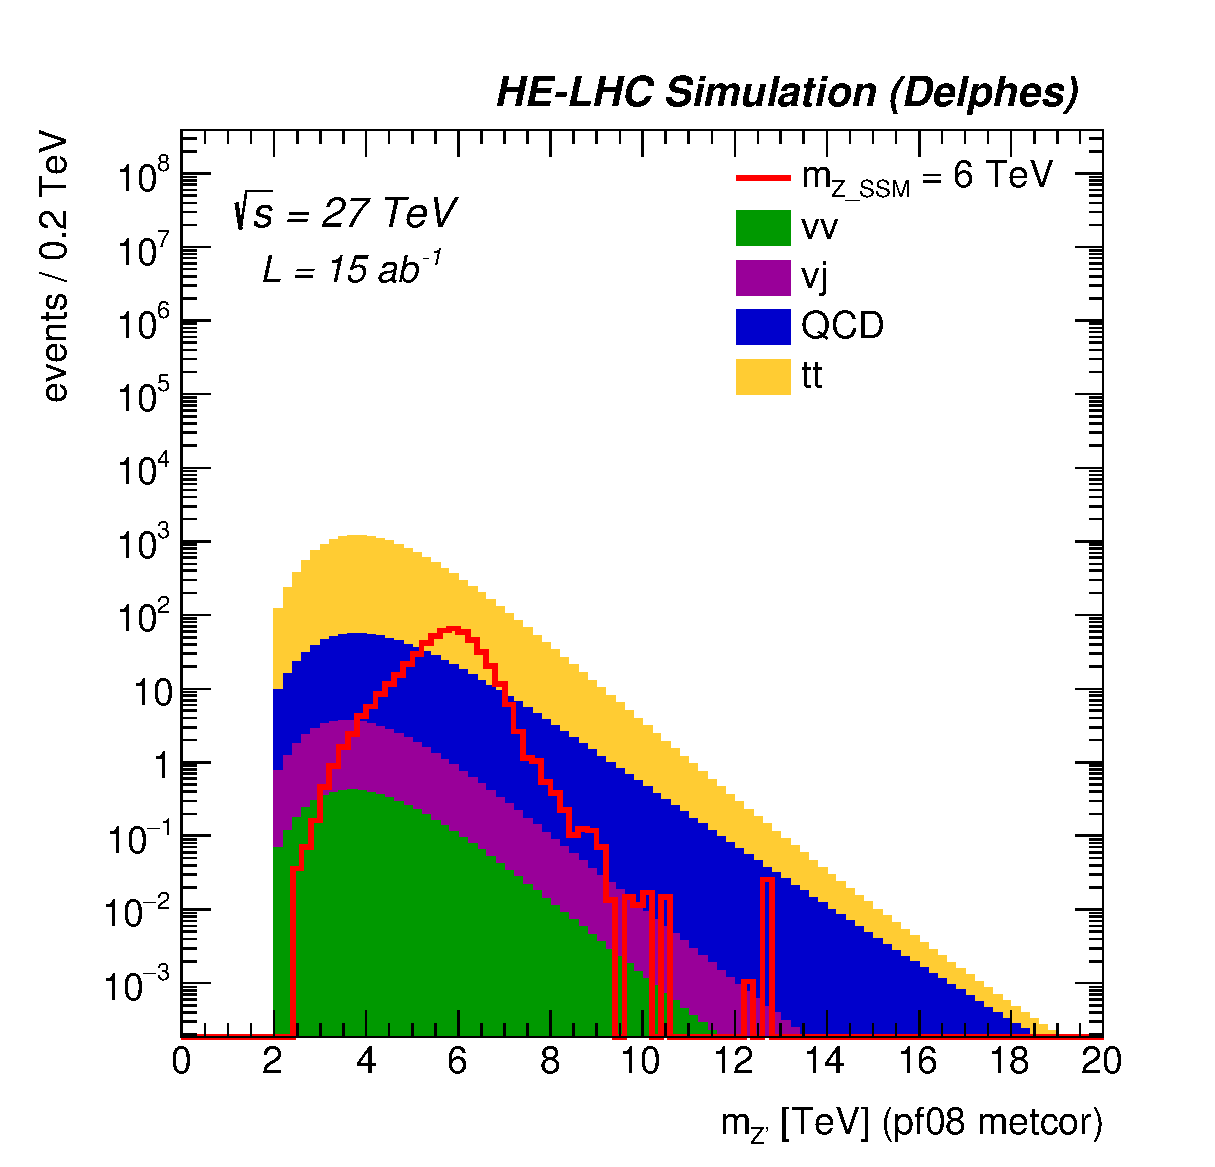
\includegraphics[width=0.30\columnwidth]{figures/Mj1j2_pf08_MetCorr_fit_sel0_nostack_log_tt.eps}
  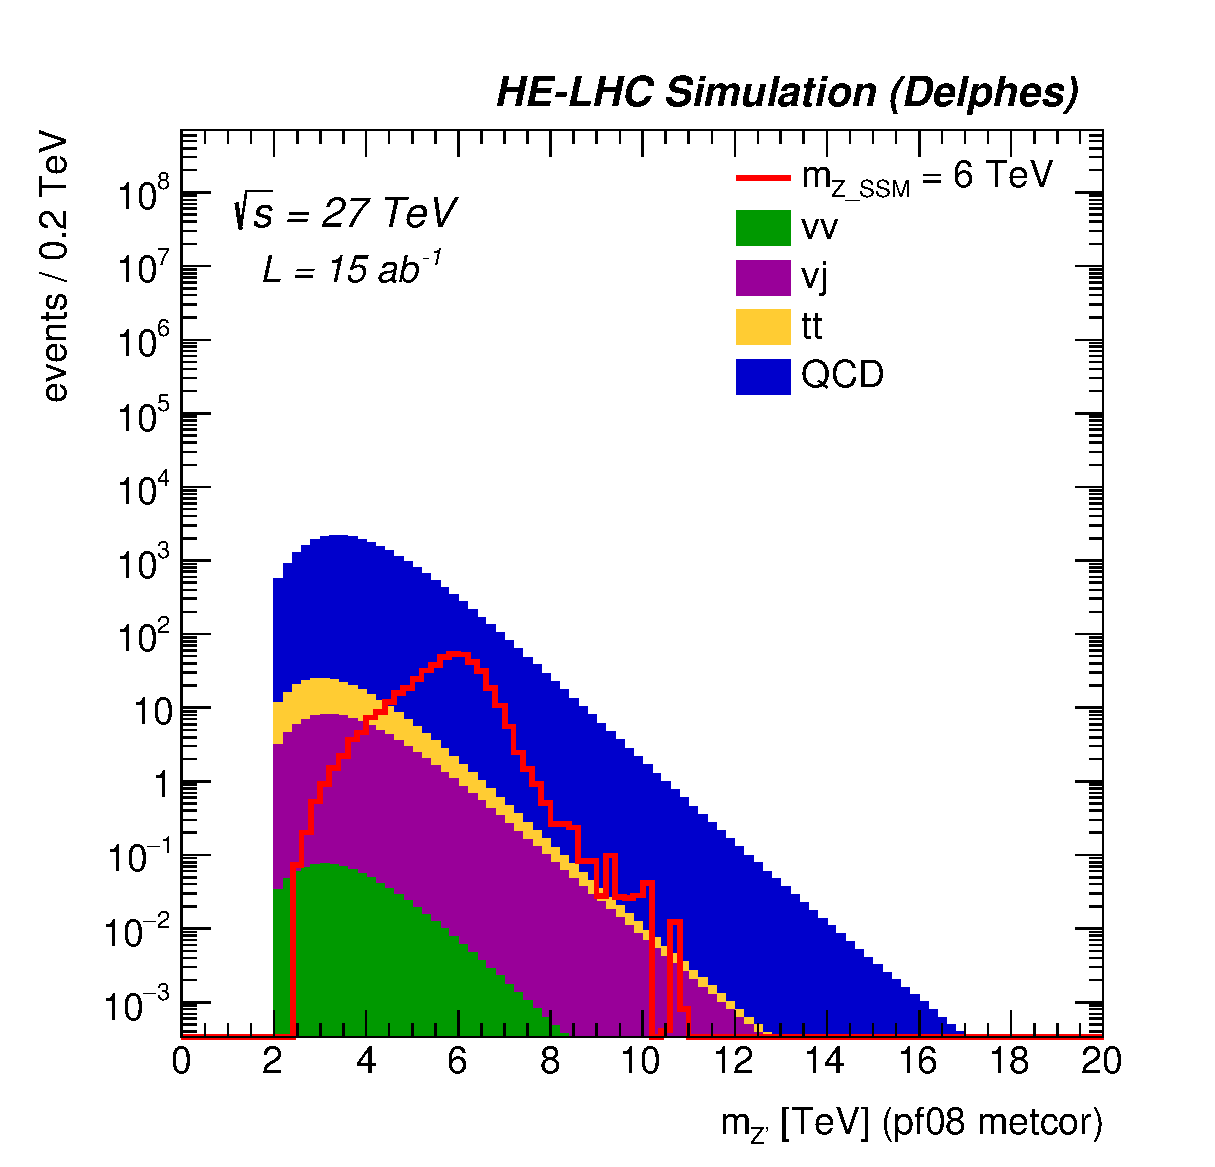
\includegraphics[width=0.30\columnwidth]{figures/Mj1j2_pf08_MetCorr_fit_sel0_nostack_log_bb.eps}
  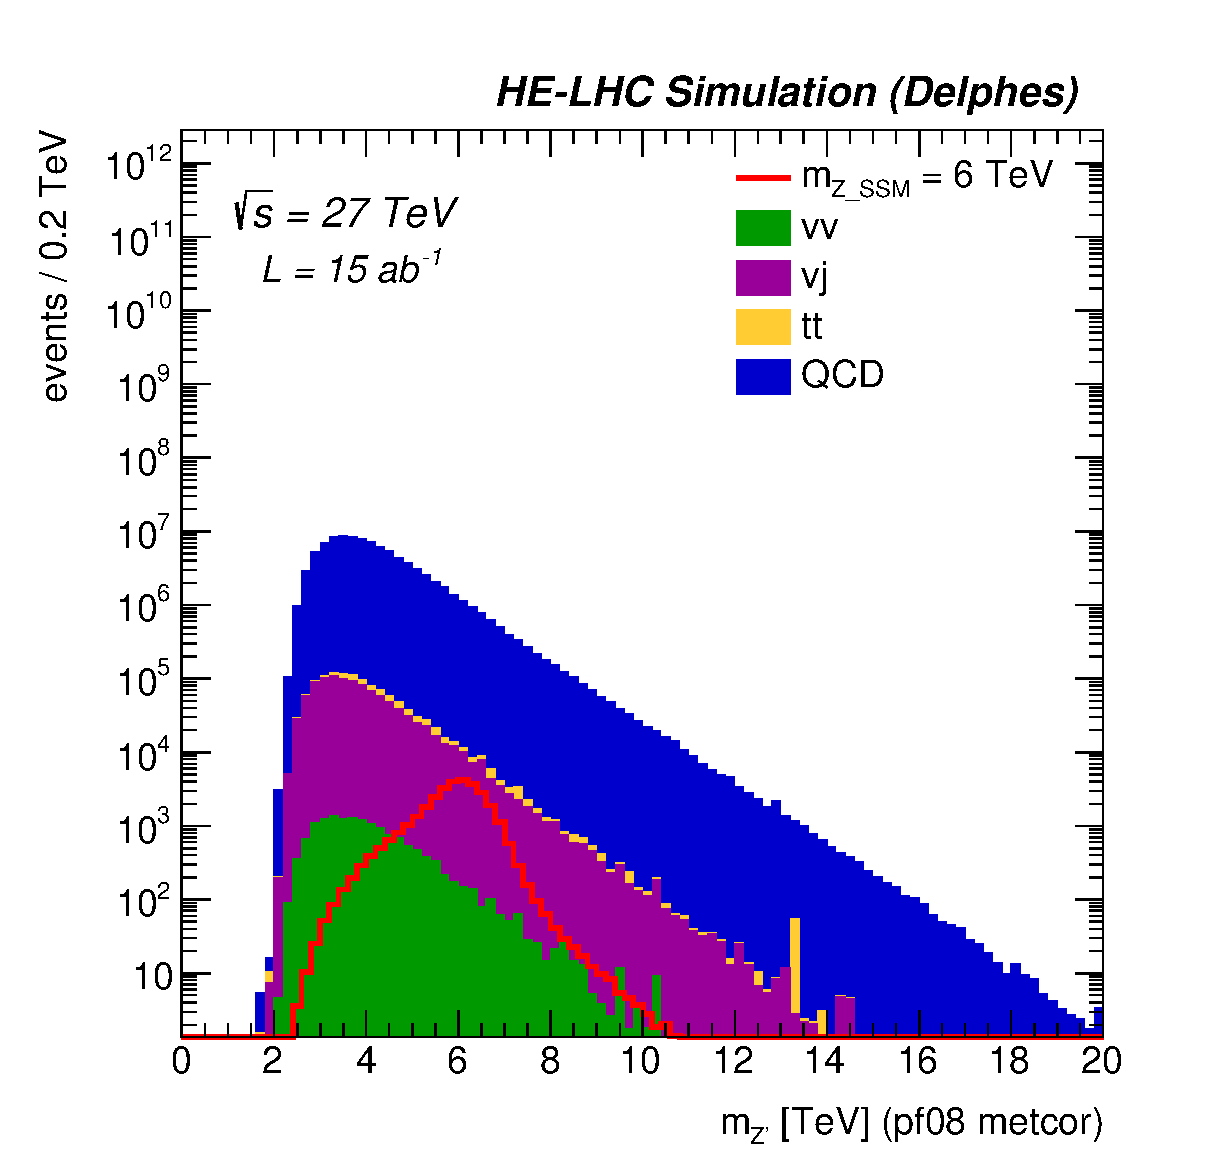
\includegraphics[width=0.30\columnwidth]{figures/Mj1j2_pf08_MetCorr_fit_sel0_nostack_log_jj.eps}
  \caption{Left, center: Invariant mass for a 6~TeV signal after full event selection for ee channel (left) and $\mu\mu$ channel (center). Right: Transverse mass for a 6~TeV signal after full event selection for the $\tau\tau$ channel. }
  \label{figure:leptonicresonances:masses}
\end{figure}

\subsubsection{Results}


\begin{figure}[h]
  \centering
     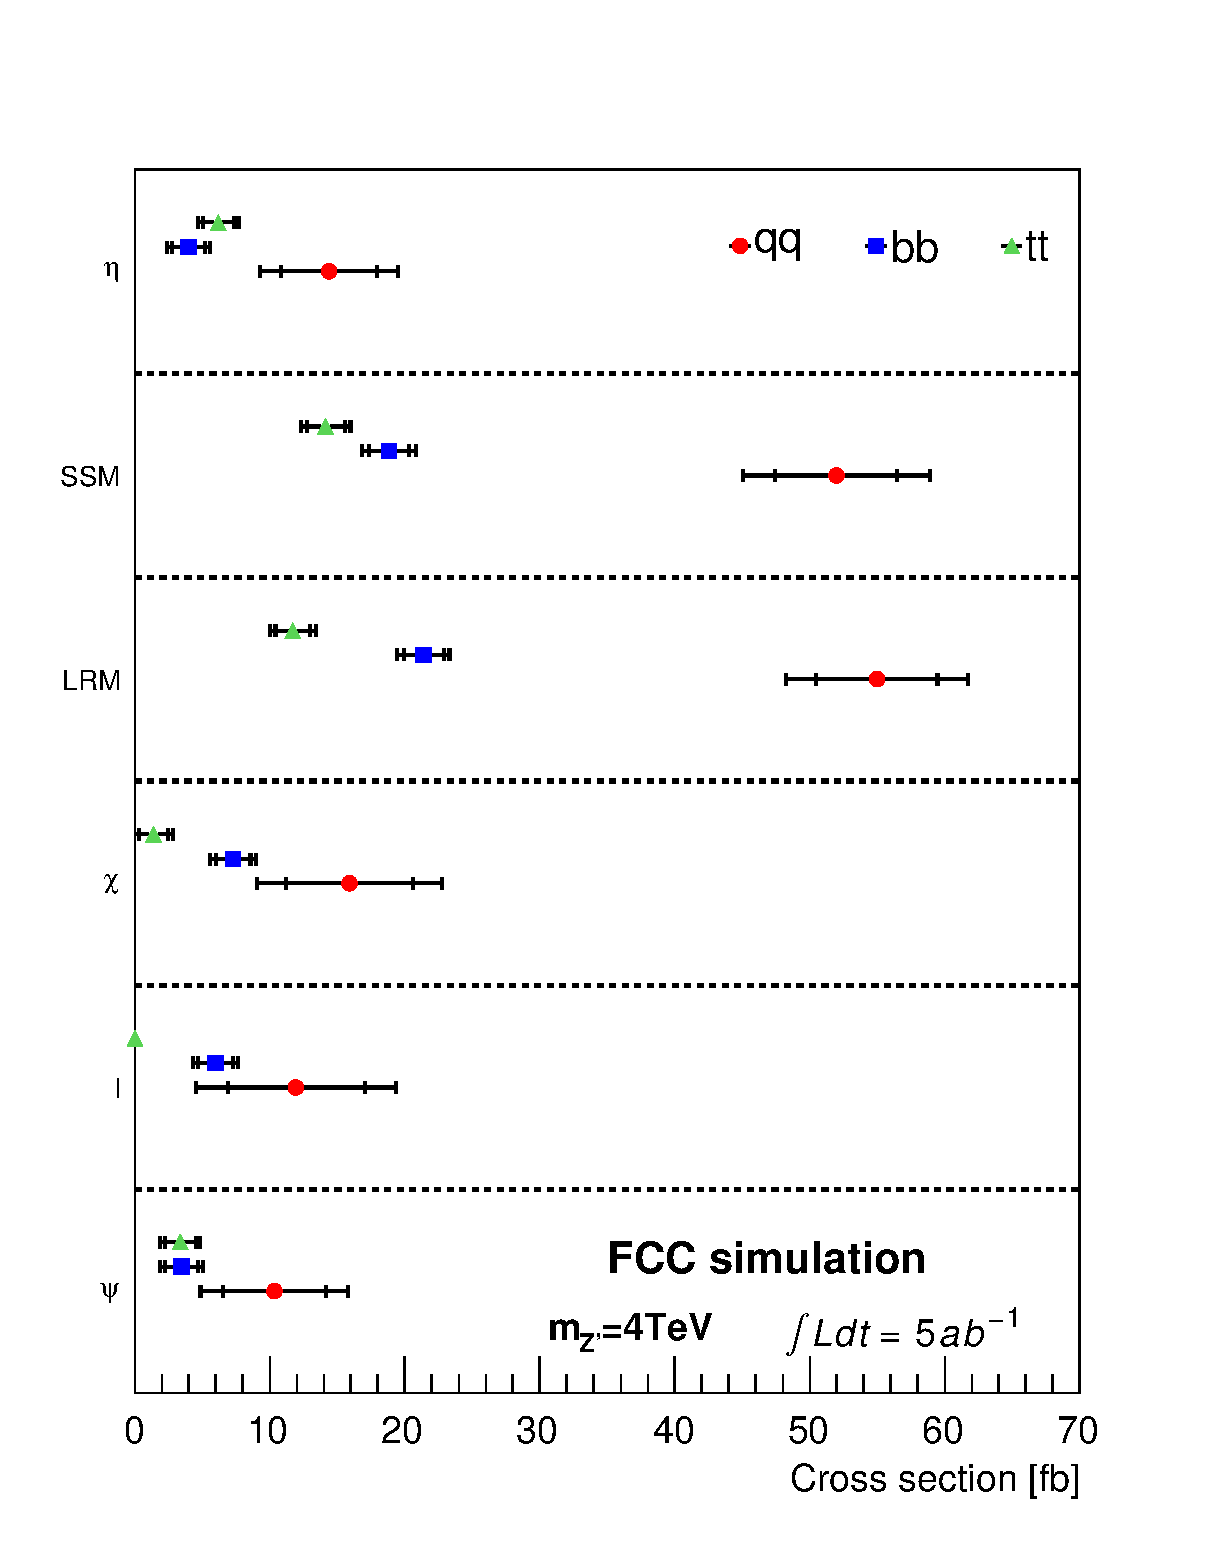
\includegraphics[width=0.3\columnwidth]{figures/Zp_branching_4TeV_5ab.eps}
    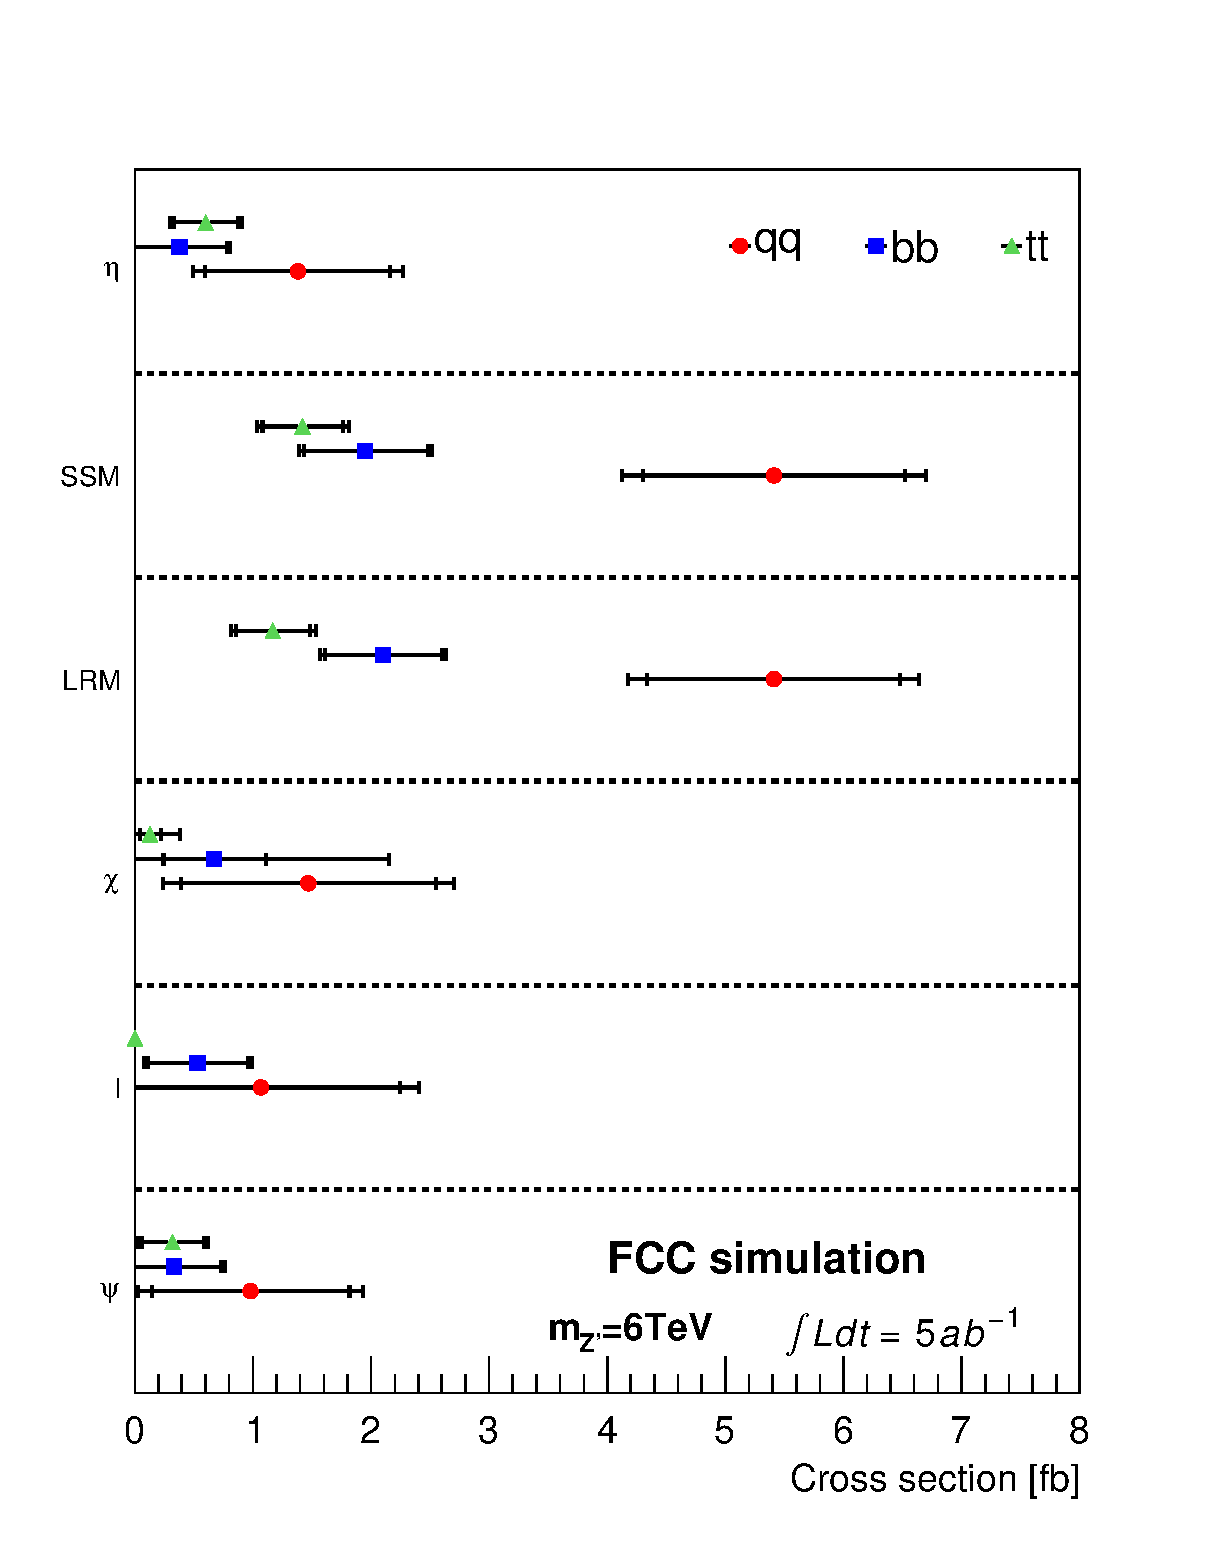
\includegraphics[width=0.3\columnwidth]{figures/Zp_branching_6TeV_5ab.eps}
    \includegraphics[width=0.3\columnwidth]{figures/Zp_branching_8TeV_5ab.eps}

    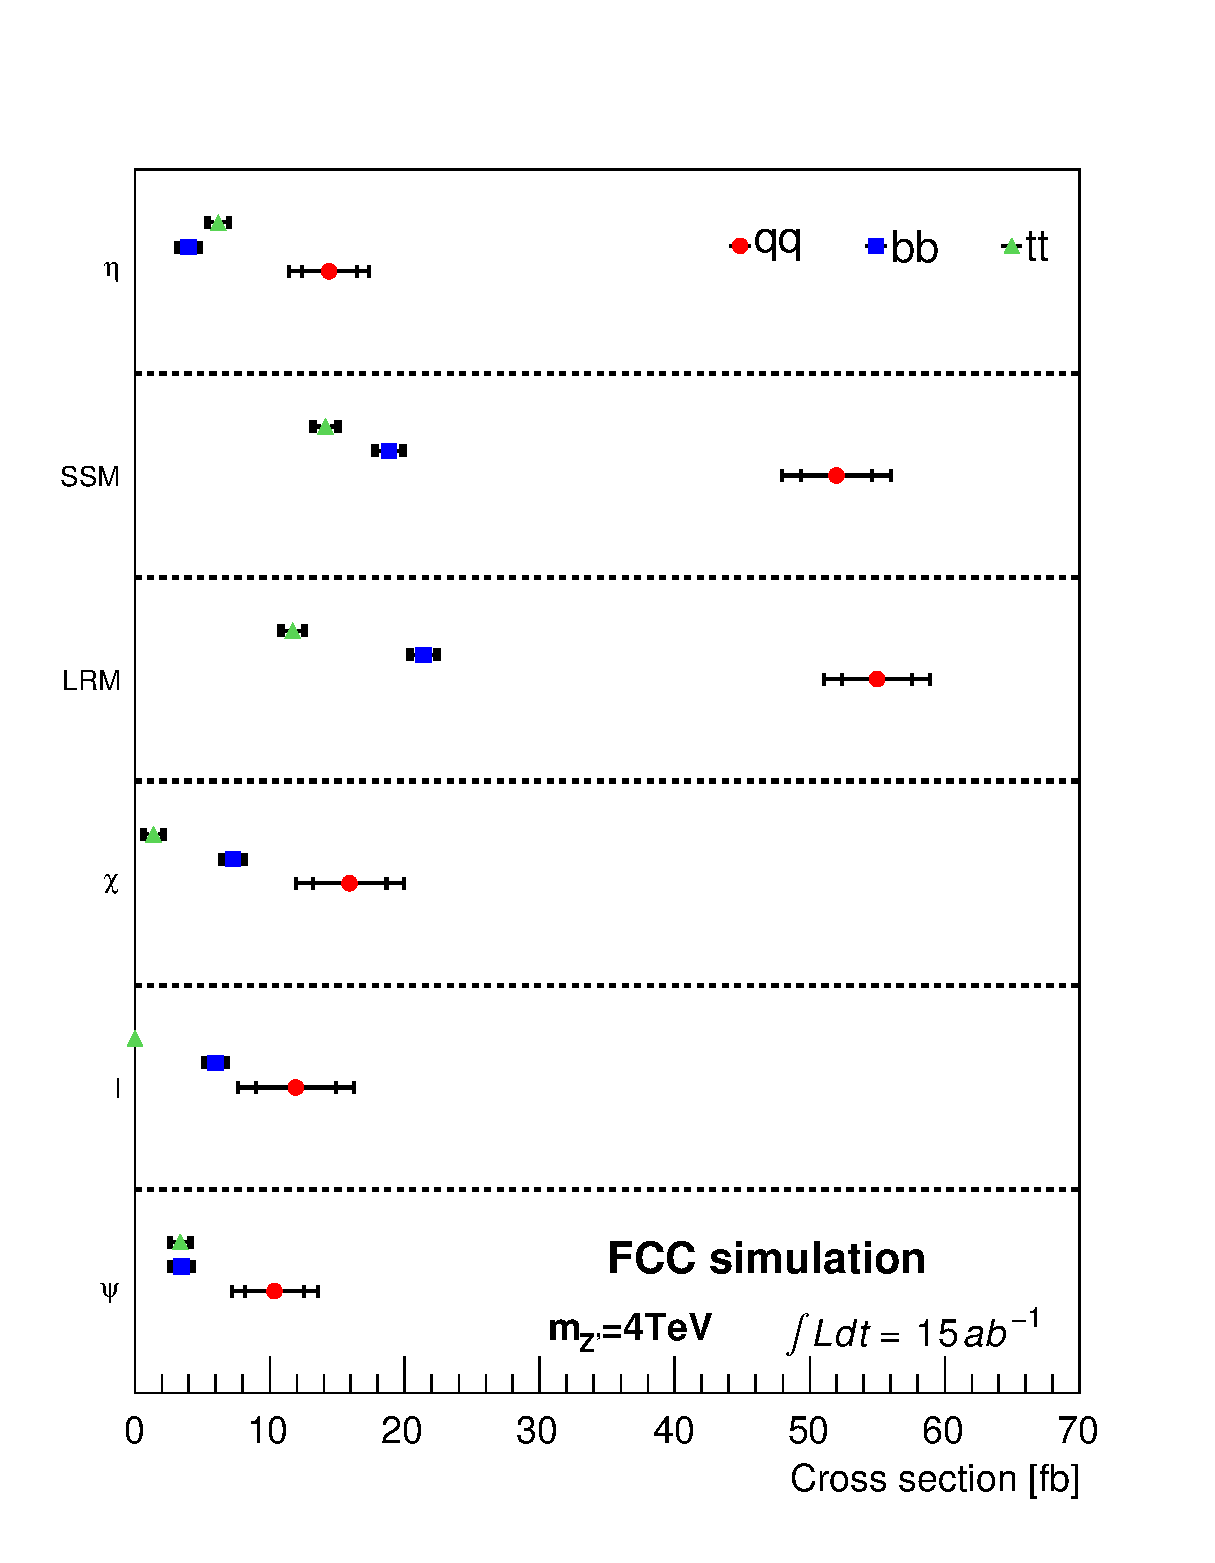
\includegraphics[width=0.3\columnwidth]{figures/Zp_branching_4TeV_15ab.eps}
    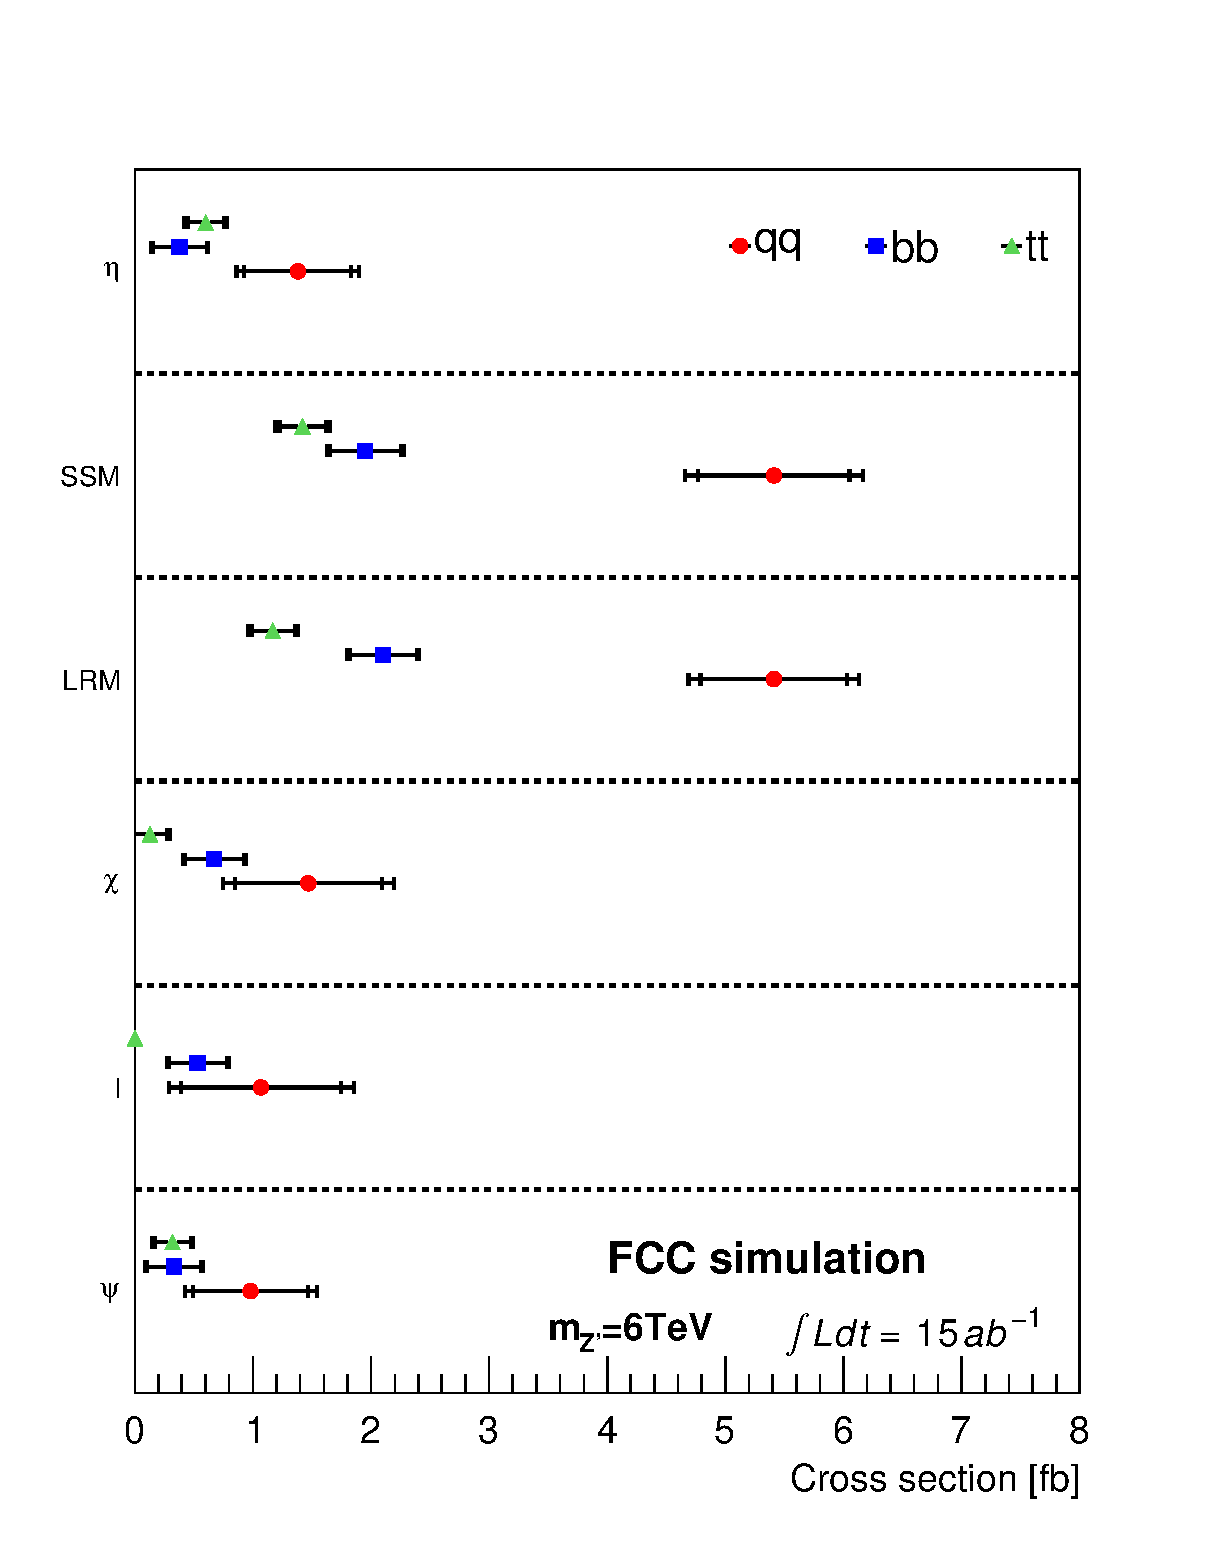
\includegraphics[width=0.3\columnwidth]{figures/Zp_branching_6TeV_15ab.eps}
    \includegraphics[width=0.3\columnwidth]{figures/Zp_branching_8TeV_15ab.eps}

    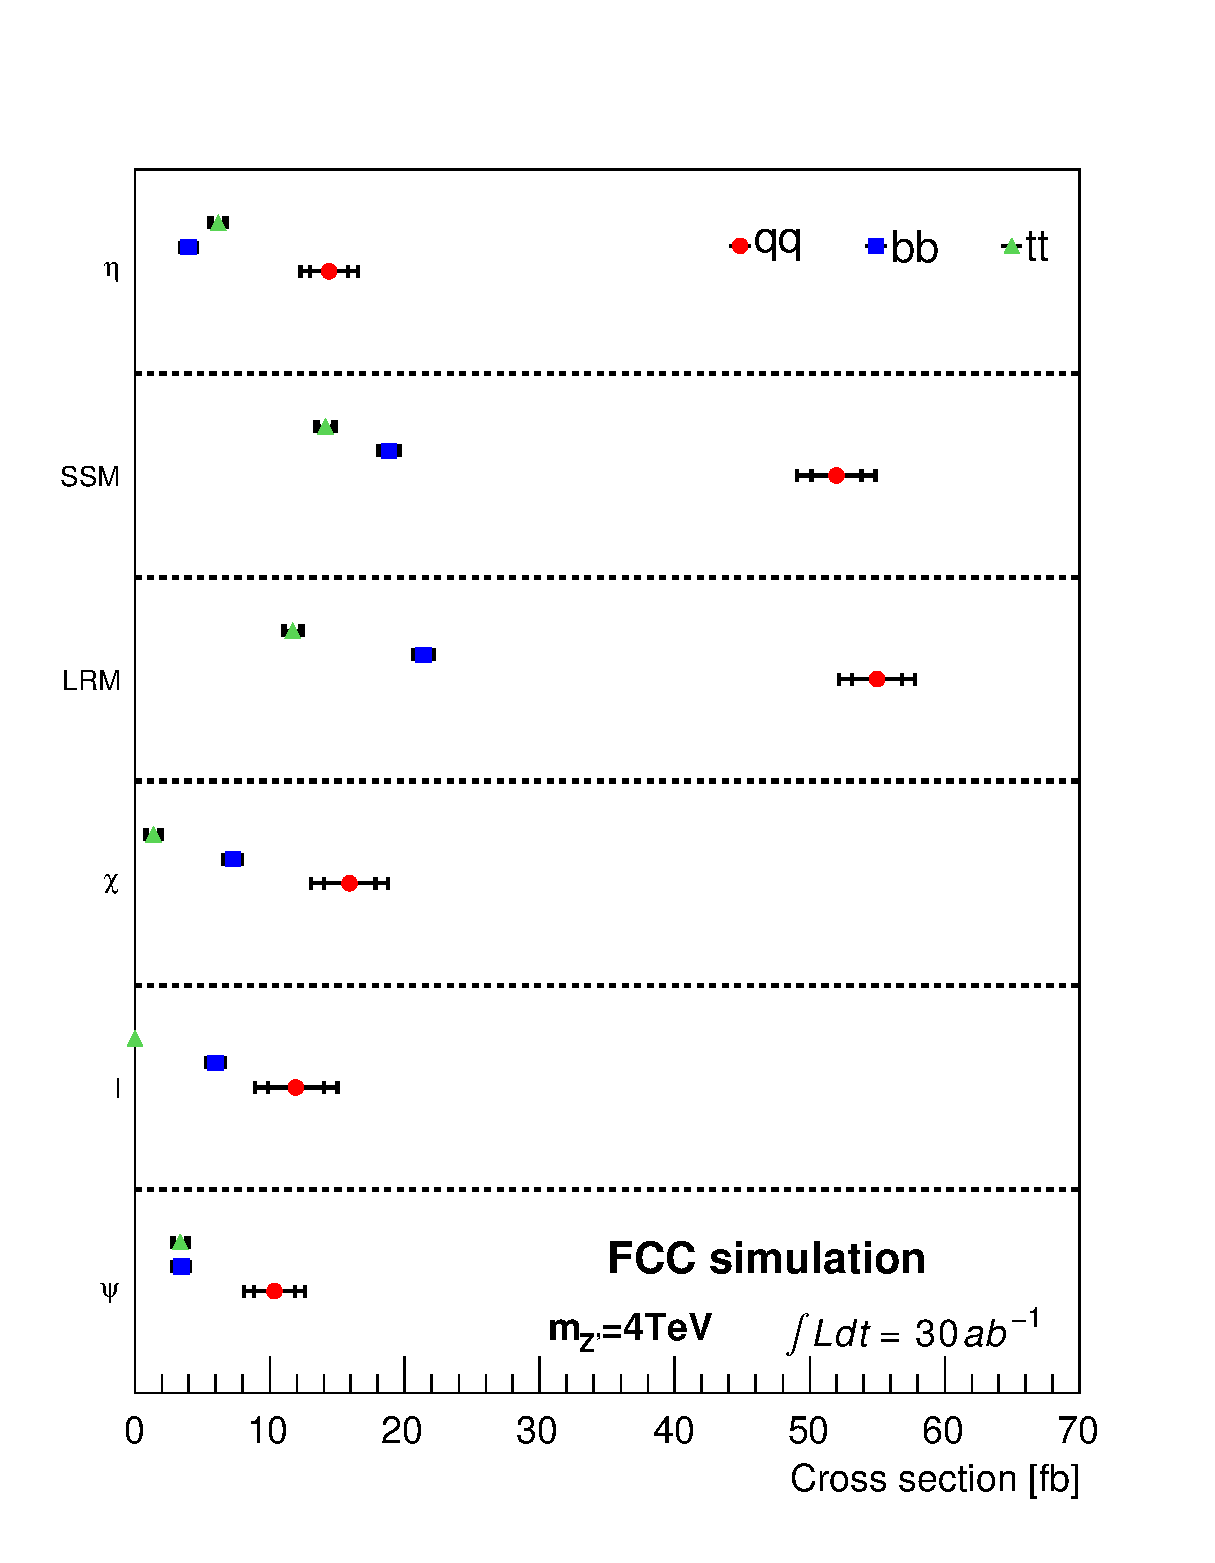
\includegraphics[width=0.3\columnwidth]{figures/Zp_branching_4TeV_30ab.eps}
    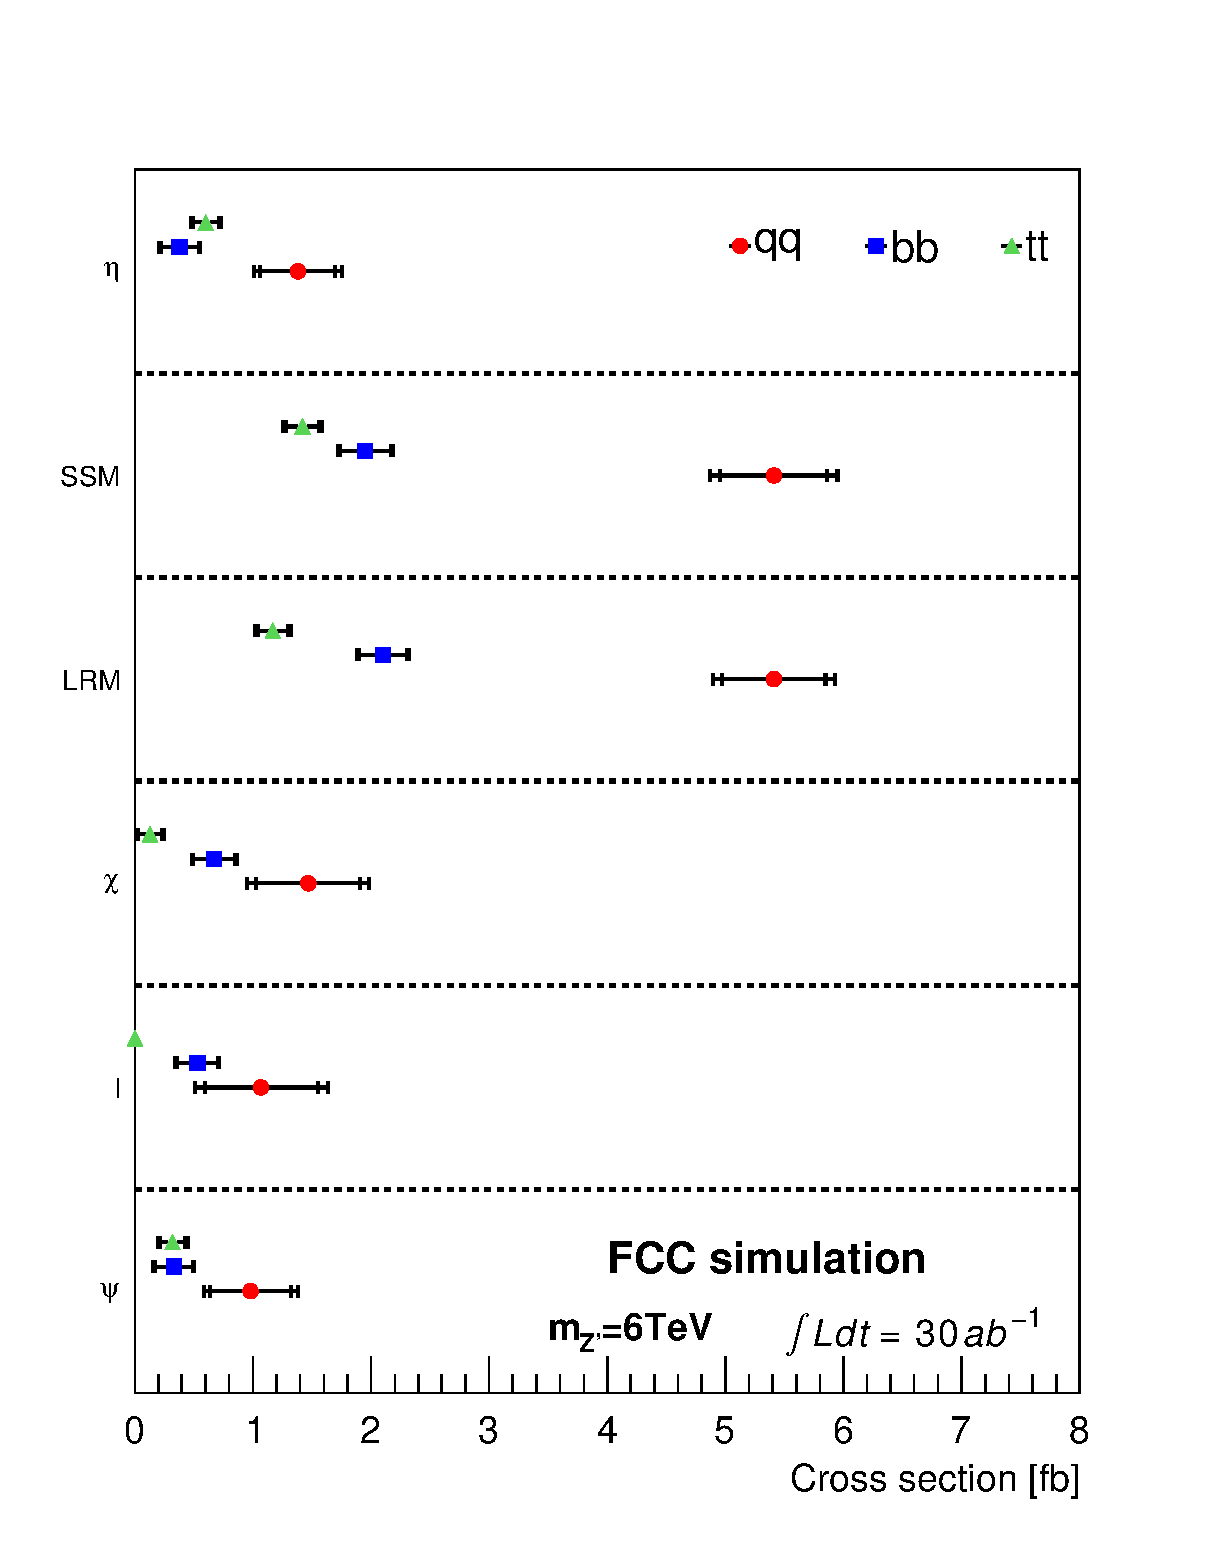
\includegraphics[width=0.3\columnwidth]{figures/Zp_branching_6TeV_30ab.eps}
    \includegraphics[width=0.3\columnwidth]{figures/Zp_branching_8TeV_30ab.eps}
  \caption{Discrimination for 4, 6 and 8TeV (left, center, right) masses with 5, 15 and 30ab$^{-1}$ (up, middle, down) of integrated luminosity. Statistical and full uncertainties are shown on each point.}
  \label{figure:hadana:discri30ab}
\end{figure}

The model discrimination achieved by the hadronic analyses for 4, 6 and 8TeV considering an integrated luminosity of 
5, 15 and 30ab$^{-1}$ respectively is shown on Fig.~\ref{figure:hadana:discri5ab}, \ref{figure:hadana:discri15ab}, \ref{figure:hadana:discri30ab}.
From the leptonic analysis~\ref{sec:lepana}, it was shown that for $r_y$ 
For all cases, except for a mass of 8TeV and an integrated luminosity of 5ab$^{-1}$, discrimination is obtained at more than one sigma for the di-jet case.


\section{Summary}


%------------------------------------ ACKNOWLEDGEMENTS ---------------------------------------%
\section*{Acknowledgements}

%
This work was supported by the Department of Energy, Contract DE-AC02-76SF00515.


%------------------------------------------- REFERENCES -------------------------------------------%


\begin{thebibliography}{99}


%\cite{Rizzo:2014xma}
\bibitem{Rizzo:2014xma} 
  T.~G.~Rizzo,
  %``Exploring new gauge bosons at a 100 TeV collider,''
  Phys.\ Rev.\ D {\bf 89}, no. 9, 095022 (2014)
  doi:10.1103/PhysRevD.89.095022
  [arXiv:1403.5465 [hep-ph]].
  %%CITATION = doi:10.1103/PhysRevD.89.095022;%%
  
%\cite{Han:2013mra}
\bibitem{Han:2013mra} 
  T.~Han, P.~Langacker, Z.~Liu and L.~T.~Wang,
  %``Diagnosis of a New Neutral Gauge Boson at the LHC and ILC for Snowmass 2013,''
  arXiv:1308.2738 [hep-ph].
  %%CITATION = ARXIV:1308.2738;%%
 
 %\cite{Harland-Lang:2014zoa}
\bibitem{Harland-Lang:2014zoa} 
  L.~A.~Harland-Lang, A.~D.~Martin, P.~Motylinski and R.~S.~Thorne,
  %``Parton distributions in the LHC era: MMHT 2014 PDFs,''
  Eur.\ Phys.\ J.\ C {\bf 75}, no. 5, 204 (2015)
  doi:10.1140/epjc/s10052-015-3397-6
  [arXiv:1412.3989 [hep-ph]].
  %%CITATION = doi:10.1140/epjc/s10052-015-3397-6;%%
  

%\cite{Aaboud:2017buh}
\bibitem{Aaboud:2017buh} 
  M.~Aaboud {\it et al.} [ATLAS Collaboration],
  %``Search for new high-mass phenomena in the dilepton final state using 36 fb$^{?1}$ of proton-proton collision data at $ \sqrt{s}=13 $ TeV with the ATLAS detector,''
  JHEP {\bf 1710}, 182 (2017)
  doi:10.1007/JHEP10(2017)182
  [arXiv:1707.02424 [hep-ex]].
  %%CITATION = doi:10.1007/JHEP10(2017)182;%%


%\cite{Sirunyan:2018exx}
\bibitem{Sirunyan:2018exx} 
  A.~M.~Sirunyan {\it et al.} [CMS Collaboration],
  %``Search for high-mass resonances in dilepton final states in proton-proton collisions at $\sqrt{s}=$ 13 TeV,''
  arXiv:1803.06292 [hep-ex].
  %%CITATION = ARXIV:1803.06292;%%


%\cite{Han:2016qpd}
\bibitem{Han:2016qpd} 
  J.~Han [ATLAS and CMS Collaborations],
  %``Dilepton Forward-Backward Asymmetry and electroweak mixing angle at ATLAS and CMS,''
  PoS ICHEP {\bf 2016}, 677 (2016).
 
 %\cite{CMS:2017zzj}
\bibitem{CMS:2017zzj} 
  CMS Collaboration [CMS Collaboration],
  %``Measurement of the weak mixing angle with the forward-backward asymmetry of Drell-Yan events at 8 TeV,''
  CMS-PAS-SMP-16-007.
  %%CITATION = CMS-PAS-SMP-16-007;%%
  
\bibitem{fccsw} FCCSW main page, http://fccsw.web.cern.ch/fccsw/

\bibitem{HELHCtwiki} HE-LHC twiki https://twiki.cern.ch/twiki/bin/view/LHCPhysics/HLHELHCWorkshop

\bibitem{Sjostrand:2014zea}
  T.~Sj�strand {\it et al.},
  %``An Introduction to PYTHIA 8.2,''
  Comput.\ Phys.\ Commun.\  {\bf 191} (2015) 159
  doi:10.1016/j.cpc.2015.01.024
  [arXiv:1410.3012 [hep-ph]].
  %%CITATION = doi:10.1016/j.cpc.2015.01.024;%%
  %1167 citations counted in INSPIRE as of 18 Sep 2018

\bibitem{Alwall:2014hca}
  J.~Alwall {\it et al.},
  %``The automated computation of tree-level and next-to-leading order differential cross sections, and their matching to parton shower simulations,''
  JHEP {\bf 1407} (2014) 079
  doi:10.1007/JHEP07(2014)079
  [arXiv:1405.0301 [hep-ph]].
  %%CITATION = doi:10.1007/JHEP07(2014)079;%%
  %3067 citations counted in INSPIRE as of 18 Sep 2018

\end{thebibliography}

%-------------------------------------------------- END --------------------------------------------------%

\end{document}



  
 


